% !TeX encoding = UTF-8
% !TeX TS-program = latexmk
% Mathematical Programming: An Introduction to Optimization
% Faithful reconstruction of source PDF pages 161--240.
% Except for the documented corrections, slide titles, prose, equations,
% examples, ordering, colors, and figure captions reproduce the source deck.
% See mathematical-programming-2026-2027-161-240-corrections.md.

\PassOptionsToPackage{cmyk}{xcolor}
\documentclass[aspectratio=169,hyperref,UTF8,CJK]{beamer}

\makeatletter
\newcommand{\beamer@scu@fontextend}{%
  \setsansfont{Latin Modern Sans}%
  \setmonofont{Latin Modern Mono}%
}
\makeatother

\usetheme[
  ColorDisplay=JXred,
  BlockDisplay=followtheme,
  CodeTheme=listing,
  LanguageMode=en,
  Miniframes=follow,
  NavigationTool=1-2-3,
  FontTheme=Custom,
  MathFont=LM,
  BIBMode=none,
  ContentMuticols=false,
  Background=SCU-Full
]{scu}

\usepackage{array}
\usepackage{booktabs}
\usepackage{mathtools}
\usepackage{multirow}
\usepackage{tabularx}

\newcommand{\R}{\mathbb{R}}
\newcommand{\trans}{\mathsf{T}}
\newcommand{\vect}[1]{\boldsymbol{#1}}

\title[Introduction to Optimization]{Introduction to Optimization}
\subtitle{Mathematical Programming}
\author[Changxi Wang]{Changxi Wang}
\institute{Sichuan University-Pittsburgh Institute\\Chengdu, China}
\date{2026--2027 Academic Year}

\AtBeginSection[]{}
\AtBeginSubsection[]{}

\begin{document}

\setcounter{framenumber}{160}

\section{Dual Linear Programming Problems}

% Source PDF page 161
\begin{frame}{Example 23}
  \begin{itemize}
    \item \textbf{Question:}
  \end{itemize}
  \begin{equation*}
    \max\quad 4w_1+w_2
  \end{equation*}
  subject to
  \begin{align*}
    2w_1-w_2 &\le 2,\\
    w_1+w_2 &\le 3,\\
    w_1 &\le 0.
  \end{align*}
\end{frame}

% Source PDF page 162
\begin{frame}{Example 23}
  \small
  \begin{itemize}
    \item The dual problem:
      \begin{equation*}
        \min\quad 2x_1+3x_2+x_3
      \end{equation*}
      subject to
      \begin{align*}
        2x_1+2x_2+x_3 &=4,\\
        -x_1+x_2 &=1,\\
        x_i&\ge0,\qquad\forall i.
      \end{align*}
    \item Adding an artificial variable:
      \begin{equation*}
        \min\quad 2x_1+3x_2+x_3+Mx_4
      \end{equation*}
      subject to
      \begin{align*}
        2x_1+2x_2+x_3 &=4,\\
        -x_1+x_2+x_4 &=1,\\
        x_i&\ge0,\qquad\forall i.
      \end{align*}
  \end{itemize}
\end{frame}

% Source PDF page 163
\begin{frame}{Example 23}
  \scriptsize
  \begin{itemize}
    \item Apply the simplex procedure:
  \end{itemize}
  \begin{equation*}
  \left[
  \begin{array}{rrrrrr|r}
   2& 2& 1& 0& 0&0&4\\
  -1& 1& 0& 1& 0&0&1\\
  -2&-3&-1& 0& 1&0&0\\
   0& 0& 0&-1& 0&1&0
  \end{array}\right]
  \xrightarrow[,A_{(4)}+A_{(2)},]{A_{(3)}+A_{(1)}}
  \left[
  \begin{array}{rrrrrr|r}
   2& 2&1&0&0&0&4\\
  -1& 1&0&1&0&0&1\\
   0&-1&0&0&1&0&4\\
  -1& 1&0&0&0&1&1
  \end{array}\right]
  \end{equation*}
  \begin{equation*}
  \xrightarrow[,A_{(4)}-A_{(2)},]{A_{(1)}-2A_{(2)},\;A_{(3)}+A_{(2)}}
  \left[
  \begin{array}{rrrrrr|r}
   4&0&1&-2&0&0&2\\
  -1&1&0& 1&0&0&1\\
  -1&0&0& 1&1&0&5\\
   0&0&0&-1&0&1&0
  \end{array}\right].
  \end{equation*}
  \begin{itemize}
    \item $z_j=a_jM+d_j+c_j$
    \item $w_1=0\cdot M+0+1=1$
    \item $w_2=-M+1+M=1$
  \end{itemize}
\end{frame}

% Source PDF page 164
\begin{frame}{Dual Linear Programming Problems}
  \small
  \begin{itemize}
    \item Constraints: equality + inequality ($\lesseqgtr$)
    \item Variables: non-restricted + non-negative + non-positive
    \item \textbf{Primal problem:}
      \begin{equation*}
        \min\quad \vect{c}_1^{\trans}\vect{x}_1+
        \vect{c}_2^{\trans}\vect{x}_2+
        \vect{c}_3^{\trans}\vect{x}_3
      \end{equation*}
      subject to
      \begin{align*}
        A_{1,1}\vect{x}_1+A_{1,2}\vect{x}_2+A_{1,3}\vect{x}_3&=\vect{b}_1,\\
        A_{2,1}\vect{x}_1+A_{2,2}\vect{x}_2+A_{2,3}\vect{x}_3&\le\vect{b}_2,\\
        A_{3,1}\vect{x}_1+A_{3,2}\vect{x}_2+A_{3,3}\vect{x}_3&\ge\vect{b}_3,\\
        \vect{x}_1\ge\vect{0},\quad \vect{x}_2\le\vect{0},\quad
        \vect{x}_3&\text{ unrestricted.}
      \end{align*}
    \item The coefficient matrix:
      \begin{equation*}
        A=\begin{bmatrix}A_{1,1}&A_{1,2}&A_{1,3}\\A_{2,1}&A_{2,2}&A_{2,3}\\A_{3,1}&A_{3,2}&A_{3,3}\end{bmatrix}.
      \end{equation*}
  \end{itemize}
\end{frame}

% Source PDF page 165. The redundant x_3 >= 0 in the source is removed:
% unrestricted x_3 has already been replaced by x_4-x_5.
\begin{frame}{Dual Linear Programming Problems}
  \scriptsize
  \begin{itemize}
    \item Unrestricted variables $\vect{x}_3=\vect{x}_4-\vect{x}_5$, where $\vect{x}_4,\vect{x}_5\ge\vect{0}$
    \item Adding/Subtracting slack variables: $\vect{x}_6,\vect{x}_7\ge\vect{0}$
    \item \textbf{Reformulated problem:}
  \end{itemize}
  \begin{equation*}
    \min\quad \vect{c}_1^{\trans}\vect{x}_1-
    \vect{c}_2^{\trans}(-\vect{x}_2)+
    \vect{c}_3^{\trans}\vect{x}_4-
    \vect{c}_3^{\trans}\vect{x}_5+
    \vect{0}^{\trans}\vect{x}_6+\vect{0}^{\trans}\vect{x}_7
  \end{equation*}
  subject to
  \begin{align*}
    A_{1,1}\vect{x}_1-A_{1,2}(-\vect{x}_2)+A_{1,3}\vect{x}_4-A_{1,3}\vect{x}_5&=\vect{b}_1,\\
    A_{2,1}\vect{x}_1-A_{2,2}(-\vect{x}_2)+A_{2,3}\vect{x}_4-A_{2,3}\vect{x}_5+\vect{x}_6&=\vect{b}_2,\\
    A_{3,1}\vect{x}_1-A_{3,2}(-\vect{x}_2)+A_{3,3}\vect{x}_4-A_{3,3}\vect{x}_5-\vect{x}_7&=\vect{b}_3,
  \end{align*}
  \begin{equation*}
    \vect{x}_1,-\vect{x}_2,\vect{x}_4,\vect{x}_5,\vect{x}_6,\vect{x}_7\ge\vect{0}.
  \end{equation*}
\end{frame}

% Source PDF page 166
\begin{frame}{Dual Linear Programming Problems}
  \small
  \begin{itemize}
    \item Dual problem:
  \end{itemize}
  \begin{equation*}
    \max\quad \vect{b}_1^{\trans}\vect{w}_1+
    \vect{b}_2^{\trans}\vect{w}_2+
    \vect{b}_3^{\trans}\vect{w}_3
  \end{equation*}
  subject to
  \begin{align*}
    A_{1,1}^{\trans}\vect{w}_1+A_{2,1}^{\trans}\vect{w}_2+A_{3,1}^{\trans}\vect{w}_3&\le\vect{c}_1,\\
    -A_{1,2}^{\trans}\vect{w}_1-A_{2,2}^{\trans}\vect{w}_2-A_{3,2}^{\trans}\vect{w}_3&\le-\vect{c}_2,\\
    A_{1,3}^{\trans}\vect{w}_1+A_{2,3}^{\trans}\vect{w}_2+A_{3,3}^{\trans}\vect{w}_3&\le\vect{c}_3,\\
    -A_{1,3}^{\trans}\vect{w}_1-A_{2,3}^{\trans}\vect{w}_2-A_{3,3}^{\trans}\vect{w}_3&\le-\vect{c}_3,\\
    \vect{w}_2&\le\vect{0},\\
    -\vect{w}_3&\le\vect{0}.
  \end{align*}
\end{frame}

% Source PDF page 167
\begin{frame}{Dual Linear Programming Problems}
  \small
  \begin{itemize}
    \item Re-organizing:
  \end{itemize}
  \begin{equation*}
    \max\quad \vect{b}_1^{\trans}\vect{w}_1+
    \vect{b}_2^{\trans}\vect{w}_2+
    \vect{b}_3^{\trans}\vect{w}_3
  \end{equation*}
  subject to
  \begin{align*}
    A_{1,1}^{\trans}\vect{w}_1+A_{2,1}^{\trans}\vect{w}_2+A_{3,1}^{\trans}\vect{w}_3&\le\vect{c}_1,\\
    A_{1,2}^{\trans}\vect{w}_1+A_{2,2}^{\trans}\vect{w}_2+A_{3,2}^{\trans}\vect{w}_3&\ge\vect{c}_2,\\
    A_{1,3}^{\trans}\vect{w}_1+A_{2,3}^{\trans}\vect{w}_2+A_{3,3}^{\trans}\vect{w}_3&=\vect{c}_3,\\
    \vect{w}_1&\text{ unrestricted},\\
    \vect{w}_2&\le\vect{0},\\
    \vect{w}_3&\ge\vect{0}.
  \end{align*}
\end{frame}

% Source PDF page 168
\begin{frame}{Dual Linear Programming Problems}
  \small
  \begin{itemize}
    \item \textcolor{blue}{P}/\textcolor{red}{D} is minimization $\longleftrightarrow$ \textcolor{red}{D}/\textcolor{blue}{P} is maximization
    \item (\# of constraints) of \textcolor{blue}{P}/\textcolor{red}{D} $=$ (\# of variables) of \textcolor{red}{D}/\textcolor{blue}{P}
    \item (Weights of objective function) of \textcolor{blue}{P}/\textcolor{red}{D} $=$ (RHS of the constraints) of \textcolor{red}{D}/\textcolor{blue}{P}
    \item $A$ of \textcolor{blue}{P}/\textcolor{red}{D} $\longleftrightarrow A^{\trans}$ of \textcolor{red}{D}/\textcolor{blue}{P}
    \item $i$-th unrestricted variable in \textcolor{blue}{P}/\textcolor{red}{D} $\longleftrightarrow$ $i$-th equality constraint in \textcolor{red}{D}/\textcolor{blue}{P}
    \item $i$-th \textcolor{red}{non-negative/non-positive variable} in ``min'' \textcolor{blue}{P}/\textcolor{red}{D} $\longrightarrow$ $i$-th ``\textcolor{red}{$\le/\ge$}'' constraint of ``max'' \textcolor{red}{D}/\textcolor{blue}{P}
    \item $j$-th \textcolor{red}{non-negative/non-positive variable} in ``max'' \textcolor{blue}{P}/\textcolor{red}{D} $\longrightarrow$ $j$-th ``\textcolor{red}{$\ge/\le$}'' constraint of ``min'' \textcolor{red}{D}/\textcolor{blue}{P}
  \end{itemize}
\end{frame}

% Source PDF page 169
\begin{frame}{Symmetric Dual Problems}
  \begin{itemize}
    \item Symmetric primal problem
      \begin{equation*}
        \min\quad \vect{c}^{\trans}\vect{x}
        \qquad\text{subject to}\qquad
        A\vect{x}\ge\vect{b},\quad \vect{x}\ge\vect{0}
      \end{equation*}
    \item Symmetric dual problem
      \begin{equation*}
        \max\quad \vect{b}^{\trans}\vect{w}
        \qquad\text{subject to}\qquad
        A^{\trans}\vect{w}\le\vect{c},\quad \vect{w}\ge\vect{0}
      \end{equation*}
  \end{itemize}
\end{frame}

% Source PDF page 170
\begin{frame}{Interpretations of Dual Problem}
  \small
  \begin{itemize}
    \item $\vect{x}$ and $\vect{w}$ are optimal:
      \begin{equation*}
        z_o=\vect{c}^{\trans}\vect{x}=\vect{b}^{\trans}\vect{w}=\sum_{i=1}^{m}b_iw_i
      \end{equation*}
    \item Let $\vect{w}$ fixed, allow $b_i$ to vary:
      \begin{equation*}
        \frac{\partial z_o}{\partial b_i}=w_i\ge0
      \end{equation*}
    \item $w_i$: the non-negative rate of change of $z_o$ w.r.t. $b_i$
  \end{itemize}
  \textbf{See Example 1}
  \begin{itemize}
    \item[$\triangle$] $w_i$: the value of a unit of material $M_i$ in manufacturing
    \item[$\triangle$] Dual problem: to minimize the value of materials on hand subject to constraints
    \item[$\triangle$] Increase or decrease supply of materials? Should consider $w_i$ (\emph{shadow prices})
  \end{itemize}
\end{frame}

% Source PDF page 171
\begin{frame}{Complementary Slackness}
  \scriptsize
  \begin{itemize}
    \item Consider the symmetric dual problems:
    \item Slack variables: $\vect{u}=[u_1,\ldots,u_m]^{\trans}$, $\vect{v}=[v_1,\ldots,v_n]^{\trans}$
    \item $P$: $\min\ \vect{c}^{\trans}\vect{x}$, $A\vect{x}-\vect{u}=\vect{b}$, $\vect{x}\ge\vect{0}$, $\vect{u}\ge\vect{0}$
    \item $D$: $\max\ \vect{b}^{\trans}\vect{w}$, $A^{\trans}\vect{w}+\vect{v}=\vect{c}$, $\vect{w}\ge\vect{0}$, $\vect{v}\ge\vect{0}$
  \end{itemize}
  \begin{block}{Complementary Slackness}
    Suppose that $[\vect{x}^{\trans},\vect{u}^{\trans}]^{\trans}$ and
    $[\vect{w}^{\trans},\vect{v}^{\trans}]^{\trans}$ are feasible solutions of
    the above $P$ and $D$, respectively. Then they are optimal if and only if
    \begin{equation*}
      \vect{v}^{\trans}\vect{x}+\vect{u}^{\trans}\vect{w}=0.
    \end{equation*}
  \end{block}
  Equivalently,
  \begin{equation*}
    \underbrace{\begin{bmatrix}\vect{v}\\\vect{u}\end{bmatrix}}_{:=\vect{r}}
    =
    \begin{bmatrix}O&-A^{\trans}\\A&O\end{bmatrix}
    \underbrace{\begin{bmatrix}\vect{x}\\\vect{w}\end{bmatrix}}_{:=\vect{s}}
    +\begin{bmatrix}\vect{c}\\-\vect{b}\end{bmatrix},
    \qquad \vect{r}\ge\vect{0},\quad\vect{s}\ge\vect{0},\quad
    \vect{r}^{\trans}\vect{s}=0.
  \end{equation*}
\end{frame}

\section{Convex and Concave Functions}

% Source PDF page 172. The missing alpha coefficient in the source's
% concavity inequality is restored.
\begin{frame}{Convex \& Concave Functions}
  \small
  \begin{itemize}
    \item $K$ is a convex set of $\R^{n\times1}$; $f:K\to\R$ is a convex function if and only if
      \begin{equation*}
        f(\alpha\vect{x}+(1-\alpha)\vect{y})
        \le \alpha f(\vect{x})+(1-\alpha)f(\vect{y}),
        \quad \vect{x},\vect{y}\in K,\quad\alpha\in[0,1].
      \end{equation*}
    \item $K$ is a convex set of $\R^{n\times1}$; $f:K\to\R$ is a concave function if and only if
      \begin{equation*}
        f(\alpha\vect{x}+(1-\alpha)\vect{y})
        \ge \alpha f(\vect{x})+(1-\alpha)f(\vect{y}),
        \quad \vect{x},\vect{y}\in K,\quad\alpha\in[0,1].
      \end{equation*}
    \item $f$ is concave $\Longleftrightarrow -f$ is convex
    \item Affine function: both convex and concave
  \end{itemize}
\end{frame}

% Source PDF page 173
\begin{frame}{Convex \& Concave Functions}
  \begin{itemize}
    \item Examples
  \end{itemize}
  \begin{columns}[T,onlytextwidth]
    \begin{column}{0.49\textwidth}
      \centering
      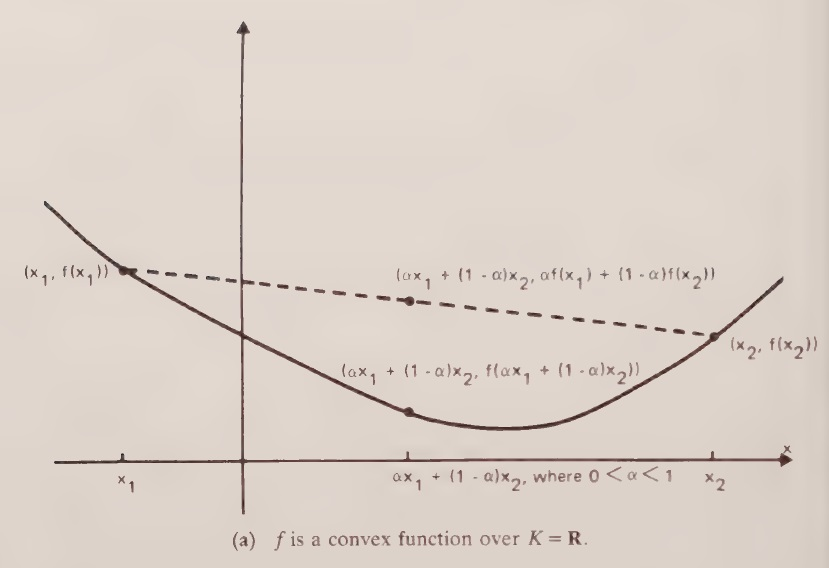
\includegraphics[width=\linewidth,height=0.53\textheight,keepaspectratio]{figures/mp-2026-pages-161-240/p173-convex-function.jpg}\\
      \small Figure 4: Convex function
    \end{column}
    \begin{column}{0.49\textwidth}
      \centering
      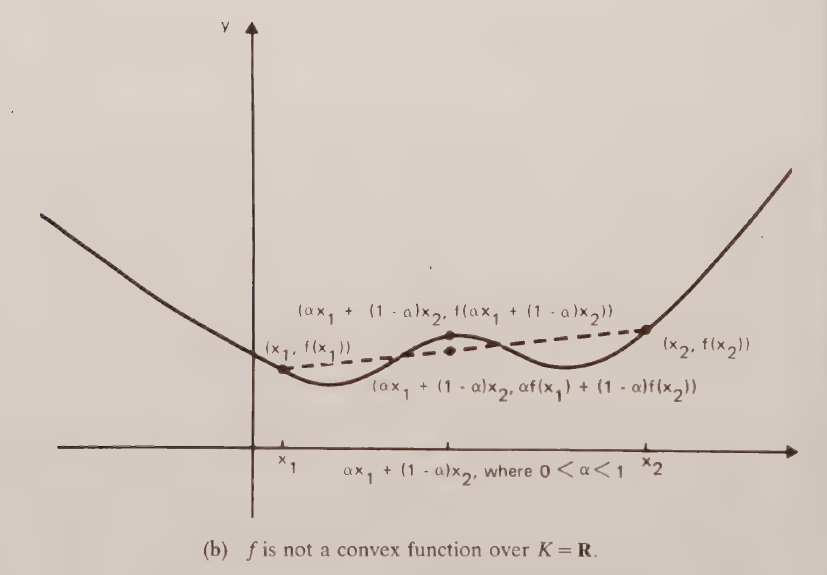
\includegraphics[width=\linewidth,height=0.53\textheight,keepaspectratio]{figures/mp-2026-pages-161-240/p173-nonconvex-function.jpg}\\
      \small Figure 5: No convex function
    \end{column}
  \end{columns}
\end{frame}

% Source PDF page 174
\begin{frame}{Convex \& Concave Functions}
  \small
  \textbf{Examples of Convex Function:}
  \begin{itemize}
    \item Any linear function: $f(\vect{x})=\vect{c}^{\trans}\vect{x}=\sum_{i=1}^{n}c_ix_i$, $K=\R^{n\times1}$
    \item Any quadratic function: $q(x)=ax^2+bx+c$, $a>0$, $K=\R$
    \item $f(x)=|x|$, where $K=\R$
    \item $f(x)=x^3$, where $K=[0,\infty)$
    \item $f([x_1,x_2]^{\trans})=4x_1^2+25x_2^2$, where $[x_1,x_2]^{\trans}\in K=\R^{2\times1}$
  \end{itemize}
  \textbf{Examples of Concave Function:}
  \begin{itemize}
    \item Any quadratic function: $q(x)=ax^2+bx+c$, $a<0$, $K=\R$
    \item $f(x)=x^3$, where $K=(-\infty,0]$
  \end{itemize}
\end{frame}

% Source PDF page 175
\begin{frame}{Convex \& Concave Functions}
  \small
  \begin{itemize}
    \item \textbf{Proposition 1}: $f:K\to\R$, $K\subseteq\R^{n\times1}$ is convex, then $f$ is a convex function if and only if
      \begin{equation*}
        f\left(\sum_{i=1}^{n}\alpha_i\vect{x}_i\right)
        \le\sum_{i=1}^{n}\alpha_i f(\vect{x}_i),
      \end{equation*}
      where $\vect{x}_i\in K$, $\alpha_i\in[0,1]$, and $\sum_{i=1}^{n}\alpha_i=1$.
    \item \textbf{Proof (sufficient condition):}

      Apparently,
      \begin{equation*}
        f\left(\sum_{i=1}^{n}\alpha_i\vect{x}_i\right)
        \le\sum_{i=1}^{n}\alpha_i f(\vect{x}_i)
        \quad\Longrightarrow\quad f\text{ is convex}.
      \end{equation*}
  \end{itemize}
\end{frame}

% Source PDF page 176
\begin{frame}{Convex \& Concave Functions}
  \small
  \begin{itemize}
    \item \textbf{Proof (necessary condition):}

      If $f$ is convex, then
      \begin{equation*}
        f(\alpha_1\vect{x}_1+\alpha_2\vect{x}_2)
        \le\alpha_1f(\vect{x}_1)+\alpha_2f(\vect{x}_2),
      \end{equation*}
      where $\vect{x}_1,\vect{x}_2\in K$, $\alpha_1,\alpha_2\in[0,1]$, $\alpha_1+\alpha_2=1$.

      Suppose the inequality holds for $n=k$; consider the convex combination
      \begin{equation*}
        \sum_{i=1}^{k+1}\alpha_i\vect{x}_i,
        \qquad \vect{x}_i\in K,\qquad
        \sum_{i=1}^{k+1}\alpha_i=1.
      \end{equation*}
  \end{itemize}
\end{frame}

% Source PDF page 177
\begin{frame}{Convex \& Concave Functions}
  \scriptsize
  Let $\alpha=\sum_{i=1}^{k}\alpha_i$; then $\alpha_{k+1}=1-\alpha$ and
  \begin{align*}
    \sum_{i=1}^{k+1}\alpha_i\vect{x}_i
      &=\sum_{i=1}^{k}\alpha_i\vect{x}_i+\alpha_{k+1}\vect{x}_{k+1}
       =\alpha\sum_{i=1}^{k}\frac{\alpha_i}{\alpha}\vect{x}_i+(1-\alpha)\vect{x}_{k+1},\\[1mm]
    f\left(\sum_{i=1}^{k+1}\alpha_i\vect{x}_i\right)
      &=f\left(\alpha\sum_{i=1}^{k}\frac{\alpha_i}{\alpha}\vect{x}_i+(1-\alpha)\vect{x}_{k+1}\right)\\
      &\le\alpha f\left(\sum_{i=1}^{k}\frac{\alpha_i}{\alpha}\vect{x}_i\right)+(1-\alpha)f(\vect{x}_{k+1})\\
      &\le\alpha\left[\sum_{i=1}^{k}\frac{\alpha_i}{\alpha}f(\vect{x}_i)\right]+(1-\alpha)f(\vect{x}_{k+1})\\
      &=\sum_{i=1}^{k}\alpha_i f(\vect{x}_i)+\alpha_{k+1}f(\vect{x}_{k+1})
       =\sum_{i=1}^{k+1}\alpha_i f(\vect{x}_i).
  \end{align*}
\end{frame}

% Source PDF page 178
\begin{frame}{Convex \& Concave Functions}
  \small
  \begin{itemize}
    \item \textbf{Proposition 2}: $K\subseteq\R^{n\times1}$ is convex, then any conical combination of convex functions defined on $K$ is a convex function defined on $K$.
    \item \textbf{Proof}: Let $f_1,\ldots,f_n$ be convex functions on $K$, and $\alpha_1\ge0,\ldots,\alpha_n\ge0$. If $\vect{x},\vect{y}\in K$ and $\alpha\in[0,1]$, then
      \begin{align*}
        \sum_{i=1}^{n}\alpha_i f_i(\alpha\vect{x}+(1-\alpha)\vect{y})
        &\le\sum_{i=1}^{n}\alpha_i\bigl[\alpha f_i(\vect{x})+(1-\alpha)f_i(\vect{y})\bigr]\\
        &=\alpha\sum_{i=1}^{n}\alpha_i f_i(\vect{x})+(1-\alpha)\sum_{i=1}^{n}\alpha_i f_i(\vect{y}).
      \end{align*}
      Thus, $\sum_{i=1}^{n}\alpha_i f_i(\vect{x})$ is a convex function.
  \end{itemize}
\end{frame}

% Source PDF page 179
\begin{frame}{Convex \& Concave Functions}
  \small
  \begin{itemize}
    \item \textbf{Proposition 3}: $f:K\to\R$ is a convex function,
      $f(K)=\{f(\vect{x}):\vect{x}\in K\}\subseteq I\subseteq\R$.
      If $g:I\to\R$ is an increasing convex function, then $(g\circ f):K\to\R$ is a convex function.
    \item \textbf{Proof}: Let $\vect{x},\vect{y}\in K$ and $\alpha\in[0,1]$:
      \begin{align*}
        (g\circ f)(\alpha\vect{x}+(1-\alpha)\vect{y})
        &=g\bigl[f(\alpha\vect{x}+(1-\alpha)\vect{y})\bigr]\\
        &\le g\bigl[\alpha f(\vect{x})+(1-\alpha)f(\vect{y})\bigr]\\
        &\le\alpha g[f(\vect{x})]+(1-\alpha)g[f(\vect{y})]\\
        &=\alpha(g\circ f)(\vect{x})+(1-\alpha)(g\circ f)(\vect{y}).
      \end{align*}
  \end{itemize}
\end{frame}

% Source PDF page 180
\begin{frame}{Example 24}
  \begin{itemize}
    \item $f([x_1,x_2]^{\trans})=4x_1^2+25x_2^2$ is convex on $\R^{2\times1}$
    \item $g(x)=x^3$ is increasing, and convex on $[0,+\infty)$
    \item $h([x_1,x_2]^{\trans})=(4x_1^2+25x_2^2)^3$ is convex
  \end{itemize}
\end{frame}
\section{Quadratic Forms and Calculus}

% Source PDF page 181. The source typo ``quadratic from'' is corrected.
\begin{frame}{Quadratic Form}
  \begin{itemize}
    \item $A=[a_{i,j}]$ is any real $n\times n$ matrix
    \item Quadratic form: $f(\vect{x})=\vect{x}^{\trans}A\vect{x}$ with $n$ variables
    \item \textcolor{blue}{Any quadratic form can be expressed as}
      \begin{align*}
        f(\vect{x})&=\vect{x}^{\trans}A\vect{x}\\
        &=\frac{1}{2}\left(\vect{x}^{\trans}A\vect{x}+\vect{x}^{\trans}A^{\trans}\vect{x}\right)\\
        &=\frac{1}{2}\vect{x}^{\trans}\underbrace{(A+A^{\trans})}_{=B}\vect{x}.
      \end{align*}
    \item $B$ is a real symmetric matrix
  \end{itemize}
\end{frame}

% Source PDF page 182
\begin{frame}{Example 25}
  \small
  \begin{itemize}
    \item $\vect{x}=[x_1,x_2,x_3]^{\trans}$
  \end{itemize}
  \begin{align*}
    f(\vect{x})
    &=x_1^2+2x_1x_2-x_1x_3+4x_2x_3-x_2^2+7x_3^2\\
    &=\begin{bmatrix}x_1&x_2&x_3\end{bmatrix}
      \begin{bmatrix}1&2&-1\\0&-1&4\\0&0&7\end{bmatrix}
      \begin{bmatrix}x_1\\x_2\\x_3\end{bmatrix}\\
    &=\begin{bmatrix}x_1&x_2&x_3\end{bmatrix}
      \frac{1}{2}\left(
      \begin{bmatrix}1&2&-1\\0&-1&4\\0&0&7\end{bmatrix}
      +\begin{bmatrix}1&0&0\\2&-1&0\\-1&4&7\end{bmatrix}\right)
      \begin{bmatrix}x_1\\x_2\\x_3\end{bmatrix}\\
    &=\begin{bmatrix}x_1&x_2&x_3\end{bmatrix}
      \begin{bmatrix}1&1&-\frac12\\1&-1&2\\-\frac12&2&7\end{bmatrix}
      \begin{bmatrix}x_1\\x_2\\x_3\end{bmatrix}.
  \end{align*}
\end{frame}

% Source PDF page 183
\begin{frame}{Quadratic Form}
  \small
  \begin{itemize}
    \item \textbf{Positive definite}: if and only if $f(\vect{x})=\vect{x}^{\trans}B\vect{x}>0$ for all nonzero $\vect{x}\in\R^n$
    \item \textbf{Positive semidefinite}: if and only if $f(\vect{x})=\vect{x}^{\trans}B\vect{x}\ge0$ for all $\vect{x}\in\R^n$
    \item \textbf{Negative definite}: if and only if $f(\vect{x})=\vect{x}^{\trans}B\vect{x}<0$ for all nonzero $\vect{x}\in\R^n$
    \item \textbf{Negative semidefinite}: if and only if $f(\vect{x})=\vect{x}^{\trans}B\vect{x}\le0$ for all $\vect{x}\in\R^n$
  \end{itemize}
\end{frame}

% Source PDF page 184. ``positive definite'' in the proof is corrected to
% ``positive semidefinite,'' matching the proposition and inequality used.
\begin{frame}{Quadratic Form}
  \scriptsize
  \begin{itemize}
    \item \textbf{Proposition 4}: Any positive/negative semidefinite quadratic form $f(\vect{x})=\vect{x}^{\trans}B\vect{x}$ is a convex/concave function.
    \item \textbf{Proof}: Due to the positive semidefinite property,
  \end{itemize}
  \begin{align*}
    f(\vect{x}-\vect{y})
      &=(\vect{x}-\vect{y})^{\trans}B(\vect{x}-\vect{y})\\
      &=\vect{x}^{\trans}B\vect{x}-\vect{x}^{\trans}B\vect{y}
        -\vect{y}^{\trans}B\vect{x}+\vect{y}^{\trans}B\vect{y}\ge0,\\[-1mm]
    &\Downarrow\\[-1mm]
    \vect{x}^{\trans}B\vect{x}+\vect{y}^{\trans}B\vect{y}
      &\ge\vect{x}^{\trans}B\vect{y}+\vect{y}^{\trans}B\vect{x}.
  \end{align*}
  Hence
  \begin{align*}
    f(\alpha\vect{x}+(1-\alpha)\vect{y})
      &=\alpha^2\vect{x}^{\trans}B\vect{x}
        +\alpha(1-\alpha)(\vect{x}^{\trans}B\vect{y}+\vect{y}^{\trans}B\vect{x})
        +(1-\alpha)^2\vect{y}^{\trans}B\vect{y}\\
      &\le\alpha^2\vect{x}^{\trans}B\vect{x}
        +\alpha(1-\alpha)(\vect{x}^{\trans}B\vect{x}+\vect{y}^{\trans}B\vect{y})
        +(1-\alpha)^2\vect{y}^{\trans}B\vect{y}\\
      &=\alpha f(\vect{x})+(1-\alpha)f(\vect{y}).
  \end{align*}
\end{frame}

% Source PDF page 185. The last line is corrected so that the convex
% combination, not the scalar function value, belongs to the level set.
\begin{frame}{Level Set}
  \small
  \begin{itemize}
    \item \textbf{Proposition 5}: If $f:K\to\R$ is convex, $K$ is a convex subset of $\R^{n\times1}$, then $\operatorname{Lev}_{\lambda}f$ is a convex set for every $\lambda\in\R$.
    \item Level set: $\operatorname{Lev}_{\lambda}f=\{\vect{x}:f(\vect{x})\le\lambda\}$
    \item \textbf{Proof}: Let $\vect{x},\vect{y}\in\operatorname{Lev}_{\lambda}f$ and $\alpha\in[0,1]$,
      \begin{equation*}
        f(\alpha\vect{x}+(1-\alpha)\vect{y})
        \le\alpha f(\vect{x})+(1-\alpha)f(\vect{y})
        \le\alpha\lambda+(1-\alpha)\lambda=\lambda.
      \end{equation*}
      Thus, $\alpha\vect{x}+(1-\alpha)\vect{y}\in\operatorname{Lev}_{\lambda}f$, which is convex.
    \item The reverse is \textbf{NOT} true
  \end{itemize}
\end{frame}

% Source PDF page 186
\begin{frame}{Epigraph}
  \scriptsize
  \begin{itemize}
    \item \textbf{Proposition 6}: $f:K\to\R$ is convex, where $K$ is a convex subset of $\R^{n\times1}$, if and only if $\operatorname{epi}(f)$ is a convex set.
    \item \emph{Epigraph}: $\operatorname{epi}(f)=\{(\vect{x},y):\vect{x}\in K,y\in\R,f(\vect{x})\le y\}$
    \item \textbf{Proof (necessary condition)}: Suppose $f$ is convex, both $(\vect{x},y)$ and $(\vect{u},v)$ belong to $\operatorname{epi}(f)$, and $\alpha\in[0,1]$.
      \begin{equation*}
        f(\alpha\vect{x}+(1-\alpha)\vect{u})
        \le\alpha f(\vect{x})+(1-\alpha)f(\vect{u})
        \le\alpha y+(1-\alpha)v.
      \end{equation*}
      Since $K$ is convex, $\alpha\vect{x}+(1-\alpha)\vect{u}\in K$, which implies
      \begin{equation*}
        \underbrace{(\alpha\vect{x}+(1-\alpha)\vect{u},\alpha y+(1-\alpha)v)}
        _{=\alpha(\vect{x},y)+(1-\alpha)(\vect{u},v)}\in\operatorname{epi}(f).
      \end{equation*}
      Hence $\operatorname{epi}(f)$ is convex.
  \end{itemize}
\end{frame}

% Source PDF page 187
\begin{frame}{Epigraph}
  \small
  \begin{itemize}
    \item \textbf{Proof (sufficient condition)}: Suppose $\operatorname{epi}(f)$ is a convex set, $\vect{x},\vect{u}\in K$, and $\alpha\in[0,1]$. Apparently, both $(\vect{x},f(\vect{x}))$ and $(\vect{u},f(\vect{u}))$ belong to $\operatorname{epi}(f)$.
      \begin{equation*}
        (\alpha\vect{x}+(1-\alpha)\vect{u},\alpha f(\vect{x})+(1-\alpha)f(\vect{u}))
        =\alpha(\vect{x},f(\vect{x}))+(1-\alpha)(\vect{u},f(\vect{u}))\in\operatorname{epi}(f).
      \end{equation*}
      \begin{equation*}
        f(\alpha\vect{x}+(1-\alpha)\vect{u})
        \le\alpha f(\vect{x})+(1-\alpha)f(\vect{u})
        \quad\Longrightarrow\quad f\text{ is convex}.
      \end{equation*}
  \end{itemize}
  \centering
  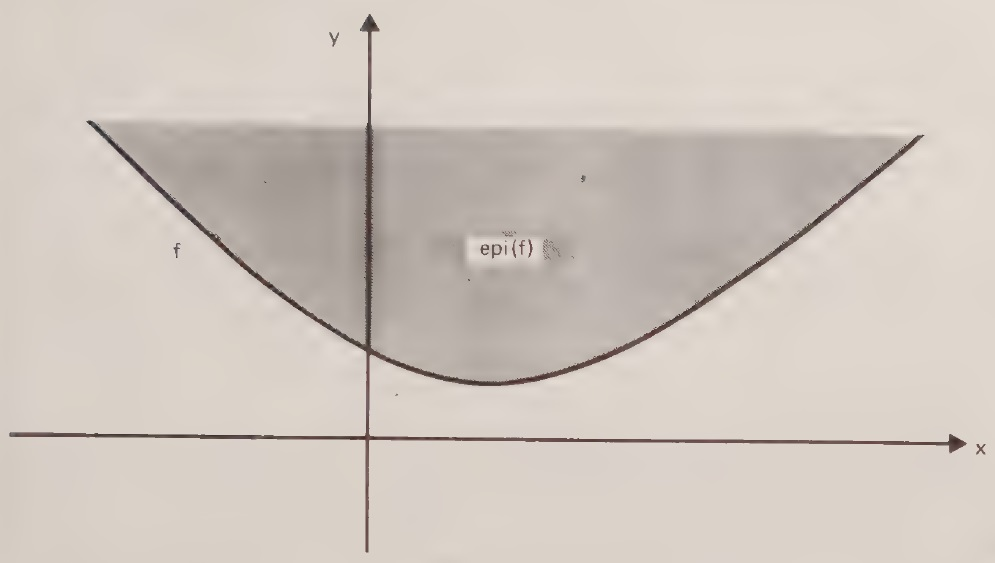
\includegraphics[width=0.48\linewidth,height=0.35\textheight,keepaspectratio]{figures/mp-2026-pages-161-240/p187-epigraph.jpg}
\end{frame}

% Source PDF page 188
\begin{frame}{Convex Functions of One Real Variable}
  \begin{itemize}
    \item \textbf{Definition}: $f:K\to\R$, and $K\subseteq\R$ is convex
    \item \emph{Derivative from the right}
      \begin{equation*}
        f_R'(x_0)=\lim_{h\to0^+}\frac{f(x_0+h)-f(x_0)}{h}
      \end{equation*}
    \item \emph{Derivative from the left}
      \begin{equation*}
        f_L'(x_0)=\lim_{h\to0^-}\frac{f(x_0+h)-f(x_0)}{h}
      \end{equation*}
    \item $f'(x_0)$ exists, if and only if $f_R'(x_0)=f_L'(x_0)=f'(x_0)$
  \end{itemize}
\end{frame}

% Source PDF page 189
\begin{frame}{Convex Functions of One Real Variable}
  \small
  \begin{itemize}
    \item \textbf{Proposition 7}: Let $I$ be an interval, and $f:I\to\R$ be a convex function. If $x_0$ is in the interior of $I$, then
      \begin{itemize}
        \item[(a)] Both $f_R'(x_0)$ and $f_L'(x_0)$ exist
        \item[(b)] $f$ is continuous at $x_0$
      \end{itemize}
    \item \textbf{Proposition 8}: Let $f:I\to\R$ be a twice continuously differentiable function over the interval $I$. $f$ is convex if and only if $f''(x)\ge0$ for every $x\in I$.
  \end{itemize}
\end{frame}

% Source PDF page 190
\begin{frame}{Some Topics from Calculus}
  \scriptsize
  \begin{itemize}
    \item $f:S\to\R$ is differentiable at interior point $\bar{\vect{x}}\in S\subseteq\R^{n\times1}$, if and only if there exist $\xi_i([\Delta x_1,\ldots,\Delta x_n]^{\trans})$ such that
      \begin{align*}
        \Delta f&=f(\bar{\vect{x}}+\Delta\vect{x})-f(\bar{\vect{x}})\\
        &=\frac{\partial f(\bar{\vect{x}})}{\partial x_1}\Delta x_1+\cdots+
          \frac{\partial f(\bar{\vect{x}})}{\partial x_n}\Delta x_n+
          \xi_1\Delta x_1+\cdots+\xi_n\Delta x_n,
      \end{align*}
      where $\xi_1\to0,\ldots,\xi_n\to0$ as $\Delta x_1\to0,\ldots,\Delta x_n\to0$.
    \item If $f$ is differentiable at $\bar{\vect{x}}$, then $f$ is continuous at $\bar{\vect{x}}$, and $\frac{\partial f(\bar{\vect{x}})}{\partial x_i}$, $\forall i$, exist.
    \item If $\frac{\partial f(\bar{\vect{x}})}{\partial x_i}$, $\forall i$, exist and are continuous over some neighborhood of $\bar{\vect{x}}$, then $f$ is continuously differentiable at $\bar{\vect{x}}$.
    \item If $\frac{\partial^2 f(\bar{\vect{x}})}{\partial x_i\partial x_j}$, $\forall i,j$, exist and are continuous over some neighborhood of $\bar{\vect{x}}$, then $f$ is twice continuously differentiable at $\bar{\vect{x}}$.
  \end{itemize}
\end{frame}

% Source PDF page 191
\begin{frame}{Directional derivative}
  \small
  \begin{itemize}
    \item \textbf{Directional derivative}: Derivative of $f$ at $\bar{\vect{x}}$ in the direction $\vect{v}$:
      \begin{equation*}
        D_{\vect{v}}f(\bar{\vect{x}})
        =\lim_{t\to0}\frac{f(\bar{\vect{x}}+t\vect{v})-f(\bar{\vect{x}})}{t}
        =\sum_{i=1}^{n}\frac{\partial f(\bar{\vect{x}})}{\partial x_i}v_i,
      \end{equation*}
      where $\vect{v}=[v_1,\ldots,v_n]^{\trans}\in\R^{n\times1}$ is a nonzero vector, and
      $L=\{\bar{\vect{x}}+t\vect{v}:t\in\R\}$ is a line in $\R^{n\times1}$ that passes through $\bar{\vect{x}}$ in the direction $\vect{v}$.
    \item Suppose $\|\vect{v}\|=1$, then $D_{\vect{v}}f(\bar{\vect{x}})$ is the slope of the tangent line at $(\bar{\vect{x}},f(\bar{\vect{x}}))$ in the cross section of the graph of $f$ with the vertical plane passing through $L$.
  \end{itemize}
\end{frame}

% Source PDF page 192
\begin{frame}{Directional derivative}
  \begin{columns}[T,onlytextwidth]
    \begin{column}{0.48\textwidth}
      \centering
      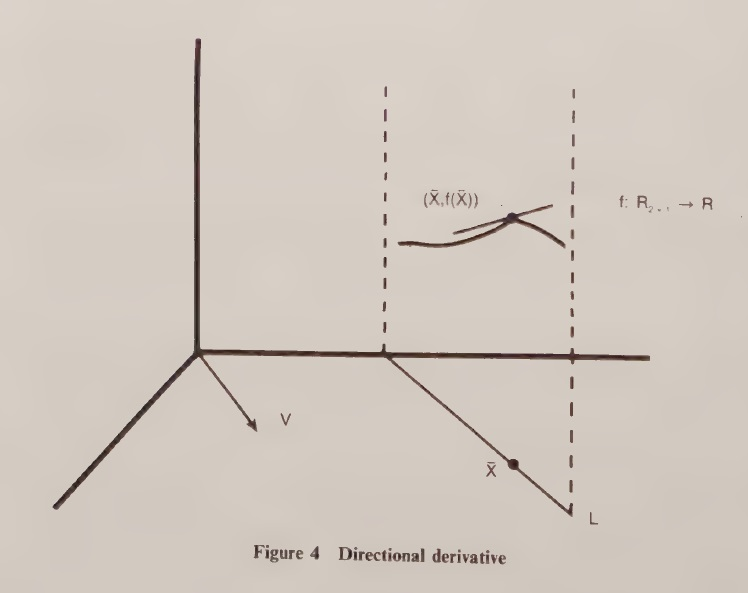
\includegraphics[width=\linewidth,height=0.56\textheight,keepaspectratio]{figures/mp-2026-pages-161-240/p192-directional-derivative.jpg}
    \end{column}
    \begin{column}{0.48\textwidth}
      \small
      \begin{itemize}
        \item $D_{\vect{v}}f(\bar{\vect{x}})$ is the instantaneous change rate of $f$ at $\bar{\vect{x}}$ in the direction of $\vect{v}$.
        \item If $\vect{v}=[0,\ldots,0,1,0,\ldots,0]^{\trans}$, where the only nonzero is in the $i$-th position, then
          \begin{equation*}
            D_{\vect{v}}f(\bar{\vect{x}})=\frac{\partial f(\bar{\vect{x}})}{\partial x_i}.
          \end{equation*}
      \end{itemize}
    \end{column}
  \end{columns}
\end{frame}

% Source PDF page 193
\begin{frame}{Gradient}
  \small
  \begin{itemize}
    \item \textbf{Gradient} of $f$ at $\bar{\vect{x}}$:
      \begin{equation*}
        \nabla f(\bar{\vect{x}})=
        \left[\frac{\partial f(\bar{\vect{x}})}{\partial x_1},\ldots,
        \frac{\partial f(\bar{\vect{x}})}{\partial x_n}\right]^{\trans}
      \end{equation*}
    \item $D_{\vect{v}}f(\bar{\vect{x}})=[\nabla f(\bar{\vect{x}})]^{\trans}\vect{v}$
    \item \textbf{Steepest ascent}:
      \begin{equation*}
        \max_{\|\vect{v}\|=1}\{D_{\vect{v}}f(\bar{\vect{x}})\}=\|\nabla f(\bar{\vect{x}})\|,
        \quad \vect{v}=\frac{\nabla f(\bar{\vect{x}})}{\|\nabla f(\bar{\vect{x}})\|}
      \end{equation*}
    \item \textbf{Steepest descent}:
      \begin{equation*}
        \min_{\|\vect{v}\|=1}\{D_{\vect{v}}f(\bar{\vect{x}})\}=-\|\nabla f(\bar{\vect{x}})\|,
        \quad \vect{v}=-\frac{\nabla f(\bar{\vect{x}})}{\|\nabla f(\bar{\vect{x}})\|}
      \end{equation*}
    \item At an interior differentiable local maximum or minimum,
      $\nabla f(\bar{\vect{x}})=\vect{0}$; such a point is called a
      \textbf{critical point}.
  \end{itemize}
\end{frame}

% Source PDF page 194
\begin{frame}{Some Topics from Calculus}
  \scriptsize
  \begin{block}{Weierstrass Theorem}
    $f:S\to\R$ is continuous, where $S$ is a closed and bounded subset of $\R^{n\times1}$; there exist points $\vect{x}^{*},\vect{y}^{*}\in S$ such that
    \begin{equation*}
      f(\vect{x}^{*})=\min\{f(\vect{x}):\vect{x}\in S\},\qquad
      f(\vect{y}^{*})=\max\{f(\vect{x}):\vect{x}\in S\}.
    \end{equation*}
  \end{block}
  \begin{itemize}
    \item \textbf{Hessian matrix (symmetric)} of $f$:
      \begin{equation*}
        H(\bar{\vect{x}})=\left[\frac{\partial^2 f(\bar{\vect{x}})}{\partial x_i\partial x_j}\right]
        =\begin{bmatrix}
        \frac{\partial^2 f}{\partial x_1^2}&\cdots&\frac{\partial^2 f}{\partial x_1\partial x_n}\\
        \vdots&\ddots&\vdots\\
        \frac{\partial^2 f}{\partial x_n\partial x_1}&\cdots&\frac{\partial^2 f}{\partial x_n^2}
        \end{bmatrix}_{\bar{\vect{x}}}.
      \end{equation*}
    \item \textbf{Generalized chain rule}: If $u=f(x_1,\ldots,x_n)$ is differentiable, and each $x_i$ is a function of $r_1,\ldots,r_m$,
      \begin{equation*}
        \frac{\partial u}{\partial r_k}=\sum_{j=1}^{n}\frac{\partial f}{\partial x_j}\frac{\partial x_j}{\partial r_k}.
      \end{equation*}
  \end{itemize}
\end{frame}

% Source PDF page 195
\begin{frame}{Some Topics from Calculus}
  \small
  \begin{block}{Taylor's Theorem}
    $f:S\to\R$ is twice continuously differentiable, where $S$ is an open convex subset of $\R^{n\times1}$. For some $\lambda\in(0,1)$,
    \begin{equation*}
      f(\vect{x})=f(\bar{\vect{x}})+[\nabla f(\bar{\vect{x}})]^{\trans}(\vect{x}-\bar{\vect{x}})
      +\frac12(\vect{x}-\bar{\vect{x}})^{\trans}
      H[\lambda\vect{x}+(1-\lambda)\bar{\vect{x}}](\vect{x}-\bar{\vect{x}}).
    \end{equation*}
  \end{block}
  \begin{itemize}
    \item There exists a function $\delta(\vect{x},\bar{\vect{x}})\to0$ as $\vect{x}\to\bar{\vect{x}}$, and
      \begin{equation*}
        f(\vect{x})=f(\bar{\vect{x}})+[\nabla f(\bar{\vect{x}})]^{\trans}(\vect{x}-\bar{\vect{x}})
        +\frac12(\vect{x}-\bar{\vect{x}})^{\trans}H(\bar{\vect{x}})(\vect{x}-\bar{\vect{x}})
        +\delta(\vect{x},\bar{\vect{x}})\|\vect{x}-\bar{\vect{x}}\|^2.
      \end{equation*}
  \end{itemize}
\end{frame}

% Source PDF page 196. ``principal minor'' is made precise as ``leading
% principal minor,'' consistent with Sylvester's criterion and the examples.
\begin{frame}{Convex Functions of Several Variables}
  \scriptsize
  \begin{itemize}
    \item \textbf{Proposition 9}: Let $f:K\to\R$ be differentiable, where $K$ is an open convex subset of $\R^{n\times1}$. Then $f$ is convex \textcolor{blue}{if and only if}
      \begin{equation*}
        f(\vect{x})-f(\vect{y})\ge[\nabla f(\vect{y})]^{\trans}(\vect{x}-\vect{y}),
        \quad\forall\vect{x},\vect{y}\in K.
      \end{equation*}
    \item \textbf{Proposition 10}: Let $f:K\to\R$ be twice continuously differentiable, where $K$ is an open convex subset of $\R^{n\times1}$. Then $f$ is convex \textcolor{blue}{if and only if} $\vect{z}^{\trans}H(\vect{y}+\lambda\vect{z})\vect{z}\ge0$ for every $\vect{y}+\lambda\vect{z}\in K$, where $\vect{y}\in K$, $\vect{z}\in\R^{n\times1}$, and $\lambda\in\R$.
    \item \textbf{Proposition 11}: For a real symmetric matrix $A=[a_{i,j}]$ to be positive definite, the \textcolor{blue}{sufficient and necessary conditions} are:
      \begin{itemize}
        \item All the eigenvalues of $A$ are positive.
        \item $a_{1,1}>0$ and each leading principal minor is positive:
          \begin{equation*}
            \begin{vmatrix}a_{1,1}&a_{1,2}\\a_{2,1}&a_{2,2}\end{vmatrix}>0,\quad
            \begin{vmatrix}a_{1,1}&a_{1,2}&a_{1,3}\\a_{2,1}&a_{2,2}&a_{2,3}\\a_{3,1}&a_{3,2}&a_{3,3}\end{vmatrix}>0,\quad\ldots,\quad |A|>0.
          \end{equation*}
      \end{itemize}
  \end{itemize}
\end{frame}

% Source PDF page 197
\begin{frame}{Example 26}
  \small
  \begin{itemize}
    \item \textbf{Question}: Examine the convexity of $f(\vect{x})=x_1^3+x_2^2+x_3$, where $\vect{x}=[x_1,x_2,x_3]^{\trans}$.
    \item \textbf{Solution}:
      \begin{equation*}
        H(\vect{x})=\begin{bmatrix}6x_1&0&0\\0&2&0\\0&0&0\end{bmatrix}.
      \end{equation*}
      \begin{equation*}
        \vect{z}^{\trans}H(\vect{x})\vect{z}=6x_1z_1^2+2z_2^2\ge0,
        \quad\forall\vect{z}=[z_1,z_2,z_3]^{\trans},
      \end{equation*}
      if and only if $x_1\ge0$. Thus, $f$ is convex over $K=\{\vect{x}:x_1\ge0\}$.
  \end{itemize}
\end{frame}

% Source PDF page 198
\begin{frame}{Example 27}
  \small
  \begin{itemize}
    \item \textbf{Question}: $f(\vect{x})=x_1^2+2x_2^2+x_3^2+3x_1-x_2+6x_3+x_2x_3-9$, where $\vect{x}=[x_1,x_2,x_3]^{\trans}$.
    \item \textbf{Solution}:
      \begin{equation*}
        H(\vect{x})=\begin{bmatrix}2&0&0\\0&4&1\\0&1&2\end{bmatrix},
      \end{equation*}
      and
      \begin{equation*}
        2>0,\qquad
        \begin{vmatrix}2&0\\0&4\end{vmatrix}>0,\qquad
        \begin{vmatrix}2&0&0\\0&4&1\\0&1&2\end{vmatrix}=14>0.
      \end{equation*}
    \item A twice continuously differentiable function over a convex set $K$ is concave if and only if $H(\vect{x})$ is negative semidefinite for each $\vect{x}\in K$.
  \end{itemize}
\end{frame}

\section{Optimization of Convex Functions}

% Source PDF page 199
\begin{frame}{Optimization of Convex Functions}
  \scriptsize
  \begin{block}{Theorem 1}
    Let $f:K\to\R$ be convex, where $K$ is a convex subset of $\R^{n\times1}$. If $f$ has a local minimum at $\bar{\vect{x}}$, then $f$ has a global minimum at $\bar{\vect{x}}$.
  \end{block}
  \begin{itemize}
    \item \textbf{Proof}: Since $\bar{\vect{x}}$ is a local minimum, there exists $\varepsilon>0$ such that $f(\bar{\vect{x}})\le f(\vect{z})$ for every $\vect{z}\in K\cap N_{\varepsilon}(\bar{\vect{x}})$. Let
      \begin{itemize}
        \item $\vect{x}\in K\setminus N_{\varepsilon}(\bar{\vect{x}})$, $\|\vect{x}-\bar{\vect{x}}\|>\varepsilon$;
        \item $0<\alpha<\frac{\varepsilon}{\|\vect{x}-\bar{\vect{x}}\|}\le1$, and let $\vect{z}=\alpha\vect{x}+(1-\alpha)\bar{\vect{x}}\in K$.
      \end{itemize}
      Then
      \begin{align*}
        \|\vect{z}-\bar{\vect{x}}\|&=\|\alpha(\vect{x}-\bar{\vect{x}})\|
        <\frac{\varepsilon}{\|\vect{x}-\bar{\vect{x}}\|}\|\vect{x}-\bar{\vect{x}}\|=\varepsilon,\\
        f(\bar{\vect{x}})&\le f(\vect{z})
        =f(\alpha\vect{x}+(1-\alpha)\bar{\vect{x}})
        \le\alpha f(\vect{x})+(1-\alpha)f(\bar{\vect{x}}),\\
        0&\le\alpha(f(\vect{x})-f(\bar{\vect{x}})).
      \end{align*}
      Hence $\bar{\vect{x}}$ is the global minimum.
  \end{itemize}
\end{frame}

% Source PDF page 200
\begin{frame}{Example 28}
  \small
  \begin{itemize}
    \item \textbf{Question}: $\min f(x)=e^{x^2}$ over $x\in K=\R$
    \item \textbf{Solution}:
      \begin{itemize}
        \item $f'(x)=2xe^{x^2}$, $f''(x)=2e^{x^2}+4x^2e^{x^2}\ge0$, $\forall x\in\R$
        \item From Proposition 8: $f$ is convex over $\R$
        \item Local minimum: Let $f'(x)=0\Longrightarrow x=0$
        \item Global minimum: At $x=0$, $f''(0)=2$
        \item Global minimum value: $f(0)=1$
      \end{itemize}
  \end{itemize}
\end{frame}

% Source PDF page 201
\begin{frame}{Optimization of Convex Functions}
  \small
  \begin{itemize}
    \item \textbf{Proposition 12}: $f:K\to\R$ is convex and continuously differentiable over a convex $K\subseteq\R^{n\times1}$. $f$ has a global minimum at $\bar{\vect{x}}$, if and only if
      \begin{equation*}
        [\nabla f(\bar{\vect{x}})]^{\trans}(\vect{x}-\bar{\vect{x}})\ge0,
        \qquad\forall\vect{x}\in K.
      \end{equation*}
    \item \textbf{Proof (sufficient condition)}:

      Suppose $[\nabla f(\bar{\vect{x}})]^{\trans}(\vect{x}-\bar{\vect{x}})\ge0$ for every $\vect{x}\in K$.
      \begin{align*}
        f\text{ is convex}
        &\Longrightarrow f(\vect{x})-f(\bar{\vect{x}})
        \ge[\nabla f(\bar{\vect{x}})]^{\trans}(\vect{x}-\bar{\vect{x}})\ge0,\\
        &\Longrightarrow f(\vect{x})\ge f(\bar{\vect{x}})\quad\text{for every }\vect{x}\in K.
      \end{align*}
  \end{itemize}
\end{frame}

% Source PDF page 202
\begin{frame}{Optimization of Convex Functions}
  \scriptsize
  \begin{itemize}
    \item \textbf{Proposition 12}: $f:K\to\R$ is convex and continuously differentiable over a convex $K\subseteq\R^{n\times1}$. $f$ has a global minimum at $\bar{\vect{x}}$ if and only if $[\nabla f(\bar{\vect{x}})]^{\trans}(\vect{x}-\bar{\vect{x}})\ge0$, $\forall\vect{x}\in K$.
    \item \textbf{Proof (necessary condition)}:

      Suppose $f$ has a global minimum at $\bar{\vect{x}}$. Let $\vect{x}\in K$.
      \begin{align*}
        &f(\bar{\vect{x}})\le f(\lambda\vect{x}+(1-\lambda)\bar{\vect{x}})
        \quad\text{for each }\lambda\in(0,1),\\
        &\frac{f(\lambda\vect{x}+(1-\lambda)\bar{\vect{x}})-f(\bar{\vect{x}})}{\lambda}
        =\frac{f(\lambda(\vect{x}-\bar{\vect{x}})+\bar{\vect{x}})-f(\bar{\vect{x}})}{\lambda}\ge0,\\
        &[\nabla f(\bar{\vect{x}})]^{\trans}(\vect{x}-\bar{\vect{x}})
        =D_{\vect{x}-\bar{\vect{x}}}f(\bar{\vect{x}})\\
        &\hspace{30mm}=\lim_{\lambda\to0^+}
        \frac{f(\lambda(\vect{x}-\bar{\vect{x}})+\bar{\vect{x}})-f(\bar{\vect{x}})}{\lambda}\ge0.
      \end{align*}
  \end{itemize}
\end{frame}

% Source PDF page 203
\begin{frame}{Optimization of Convex Functions}
  \scriptsize
  \begin{block}{Theorem 2}
    Let $f:K\to\R$ be a convex function, where $K\subseteq\R^{n\times1}$ is a convex polytope. Then $f$ has a global maximum occurring at one or more of the extreme points of $K$.
  \end{block}
  \begin{itemize}
    \item \textbf{Proof}: The finite basis theorem implies a finite number of extreme points of $K$, $\vect{x}_1,\ldots,\vect{x}_m$, exists such that
      \begin{equation*}
        K=X(\{\vect{x}_1,\ldots,\vect{x}_m\}).
      \end{equation*}
      Let $f(\bar{\vect{x}})=\max\{f(\vect{x}_i):i=1,\ldots,m\}$ and
      $\vect{x}=\sum_{i=1}^{m}\alpha_i\vect{x}_i$, where
      $\sum_{i=1}^{m}\alpha_i=1$ and $\alpha_i\in[0,1]$, $\forall i$. Then
      \begin{align*}
        f(\vect{x})=f\left(\sum_{i=1}^{m}\alpha_i\vect{x}_i\right)
        &\le\sum_{i=1}^{m}\alpha_i f(\vect{x}_i)
        \le\sum_{i=1}^{m}\alpha_i f(\bar{\vect{x}})\\
        &=f(\bar{\vect{x}})\sum_{i=1}^{m}\alpha_i=f(\bar{\vect{x}}).
      \end{align*}
  \end{itemize}
\end{frame}

% Source PDF page 204
\begin{frame}{Example 29}
  \scriptsize
  \begin{itemize}
    \item \textbf{Question}: $\max\{2x_1^2+x_2^4\}$ subject to
      \begin{align*}
        -x_1+2x_2&\le10,\\
        5x_1+3x_2&\le41,\\
        2x_1-3x_2&\le8,\\
        x_i&\ge0,\quad\forall i.
      \end{align*}
    \item \textbf{Solution}:
      \begin{itemize}
        \item Let $f(\vect{x})=2x_1^2+x_2^4$, $\frac{\partial f}{\partial x_1}=4x_1$, and $\frac{\partial f}{\partial x_2}=4x_2^3$.
        \item $H(\vect{x})=\begin{bmatrix}4&0\\0&12x_2^2\end{bmatrix}$,
          $\vect{z}^{\trans}H(\vect{x})\vect{z}=4z_1^2+12x_2^2z_2^2$ for every $\vect{z}\in\R^{2\times1}$; $f$ is convex over $\R^{2\times1}$.
        \item Let $K$ be a feasible set, which is a convex polytope with extreme points $[7,2]^{\trans}$, $[4,7]^{\trans}$, $[4,0]^{\trans}$, $[0,5]^{\trans}$, and $[0,0]^{\trans}$.
        \item The global maximum of $f$ must be one of the extreme points, i.e., $f([4,7]^{\trans})=2433$ by calculation.
      \end{itemize}
  \end{itemize}
\end{frame}

\section{Quasiconvexity and Star-shaped Sets}

% Source PDF page 205
\begin{frame}{Quasiconvex Functions}
  \small
  \begin{itemize}
    \item Let $f:K\to\R$ be over a convex $K\subseteq\R^{n\times1}$.
    \item \textcolor{blue}{Quasiconvex}: if and only if
      \begin{equation*}
        f(\alpha\vect{x}+(1-\alpha)\vect{y})
        \le\max\{f(\vect{x}),f(\vect{y})\},
        \quad\vect{x},\vect{y}\in K,\quad\alpha\in(0,1).
      \end{equation*}
    \item \textcolor{blue}{Quasiconcave}: if and only if
      \begin{equation*}
        f(\alpha\vect{x}+(1-\alpha)\vect{y})
        \ge\min\{f(\vect{x}),f(\vect{y})\},
        \quad\vect{x},\vect{y}\in K,\quad\alpha\in(0,1).
      \end{equation*}
    \item $f$ is \textbf{strongly quasiconvex/quasiconcave} when the inequality is strict.
    \item Quasiconvex/Quasiconcave $\Longleftarrow$ Convex/Concave; the converse does not hold in general.
  \end{itemize}
\end{frame}

% Source PDF page 206
\begin{frame}{Quasiconvex Functions}
  \centering
  \begin{columns}[T,onlytextwidth]
    \begin{column}{0.49\textwidth}
      \centering
      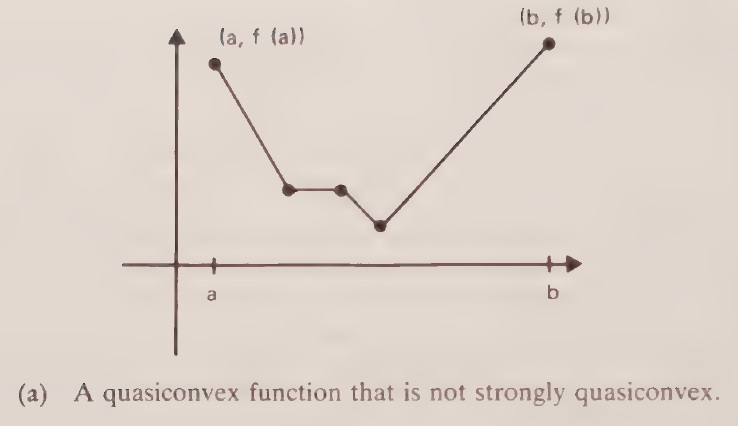
\includegraphics[width=\linewidth,height=0.66\textheight,keepaspectratio]{figures/mp-2026-pages-161-240/p206-quasiconvex.jpg}
    \end{column}
    \begin{column}{0.49\textwidth}
      \centering
      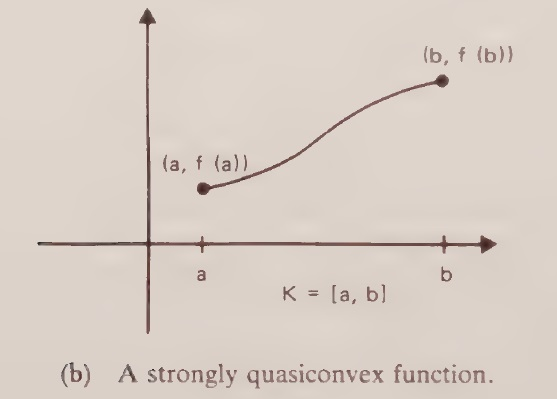
\includegraphics[width=\linewidth,height=0.66\textheight,keepaspectratio]{figures/mp-2026-pages-161-240/p206-strongly-quasiconvex.jpg}
    \end{column}
  \end{columns}
\end{frame}

% Source PDF page 207
\begin{frame}{Quasiconvex Functions}
  \scriptsize
  \begin{itemize}
    \item[$\star$] Let $f:K\to\R$, and convex $K\subseteq\R^{n\times1}$.
    \item \textbf{Proposition 13}: $f$ is quasiconvex over $K$, if and only if $\operatorname{Lev}_{\lambda}f$ is convex $\forall\lambda\in\R$.
      \begin{itemize}
        \item \textbf{Corollary}: if and only if, for each $\vect{x}_i\in K$, $\alpha_i\ge0$, $\sum_{i=1}^{n}\alpha_i=1$, and $n\in\mathbb{N}$,
          \begin{equation*}
            f\left(\sum_{i=1}^{n}\alpha_i\vect{x}_i\right)
            \le\max\{f(\vect{x}_i):i=1,\ldots,n\}.
          \end{equation*}
      \end{itemize}
    \item \textbf{Proposition 14}: $f$ is quasiconvex over a polytope $K$, then $f$ has a global maximum at an extreme point of $K$.
      \begin{itemize}
        \item An extension of theorem 2 for convex function.
      \end{itemize}
    \item \textbf{Proposition 15}: $f$ is strongly quasiconvex over $K$. If $f$ has a local minimum at $\bar{\vect{x}}$, then $f$ has a global minimum at $\bar{\vect{x}}$.
  \end{itemize}
\end{frame}

% Source PDF page 208
\begin{frame}{Star-shaped at a Point}
  \small
  \begin{itemize}
    \item \textcolor{red}{$K$ is star-shaped at $\bar{\vect{x}}$}: $\alpha\vect{x}+(1-\alpha)\bar{\vect{x}}\in K$, for any $\vect{x}\in K$ and $\alpha\in(0,1)$.
    \item \textcolor{blue}{$f$ is convex at $\bar{\vect{x}}$}: if and only if
      \begin{equation*}
        f(\alpha\vect{x}+(1-\alpha)\bar{\vect{x}})
        \le\alpha f(\vect{x})+(1-\alpha)f(\bar{\vect{x}})
      \end{equation*}
      for any $\vect{x}\in K$ (\textcolor{red}{star-shaped at $\bar{\vect{x}}$}) and $\alpha\in(0,1)$.
    \item $f$ is convex $\Longrightarrow$ $f$ is convex at any $\bar{\vect{x}}\in K$; the converse need not hold.
    \item \textbf{Proposition 16}: $f$ has a local minimum at $\bar{\vect{x}}$ over $K$. If $K$ is \textcolor{red}{star-shaped at $\bar{\vect{x}}$} and $f$ is \textcolor{blue}{convex at $\bar{\vect{x}}$}, then $f$ has a global minimum at $\bar{\vect{x}}$.
  \end{itemize}
\end{frame}

% Source PDF page 209
\begin{frame}{Star-shaped at a Point}
  \centering
  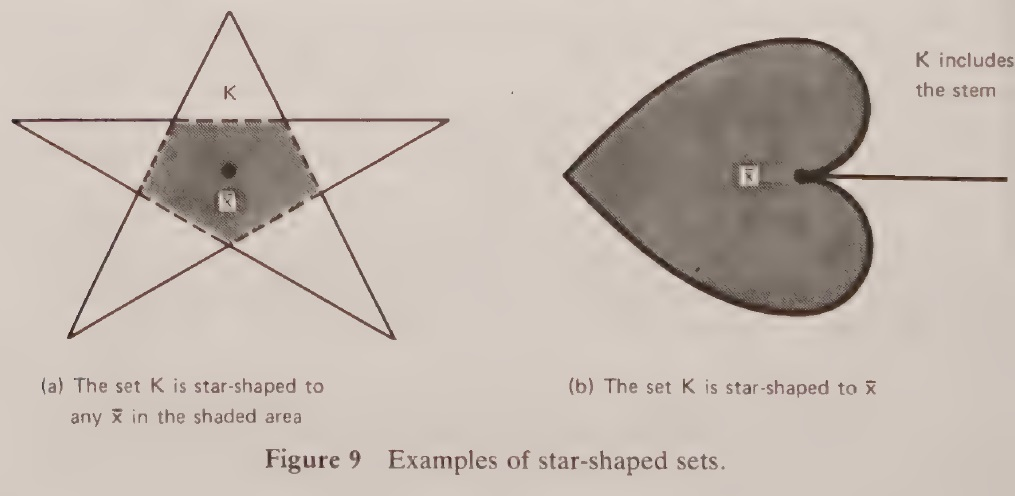
\includegraphics[width=0.86\linewidth,height=0.69\textheight,keepaspectratio]{figures/mp-2026-pages-161-240/p209-star-shaped-sets.jpg}
\end{frame}

\section{Unconstrained and Constrained Problems}

% Source PDF page 210
\begin{frame}{Unconstrained Problems}
  \small
  \begin{itemize}
    \item Consider the problem
      \begin{equation*}
        \max\ f(\vect{x}),\qquad f:\R^{n\times1}\to\R.
      \end{equation*}
    \item Suppose $\vect{x}^{*}$ is a local maximum, and $f$ is twice continuously differentiable in a neighborhood $N_{\varepsilon}(\vect{x}^{*})$ of $\vect{x}^{*}$.
    \item Thus for every direction vector $\vect{v}$, where $\|\vect{v}\|=1$,
      \begin{equation*}
        D_{\vect{v}}f(\vect{x}^{*})=
        \lim_{t\to0}\frac{f(\vect{x}^{*}+t\vect{v})-f(\vect{x}^{*})}{t}
        =[\nabla f(\vect{x}^{*})]^{\trans}\vect{v}=0.
      \end{equation*}
    \item The \textbf{1st necessary condition} for local maximum:
      \begin{equation*}
        \nabla f(\vect{x}^{*})=\vect{0}.
      \end{equation*}
  \end{itemize}
\end{frame}

% Source PDF page 211
\begin{frame}{Unconstrained Problems}
  \small
  \begin{itemize}
    \item By Taylor's theorem,
      \begin{align*}
        f(\vect{x}^{*})\ge f(\vect{x})=f(\vect{x}^{*}+t\vect{v})
        &=f(\vect{x}^{*})+t[\nabla f(\vect{x}^{*})]^{\trans}\vect{v}
          +\frac{t^2}{2}\vect{v}^{\trans}H(\vect{x}^{*}+\lambda t\vect{v})\vect{v}\\
        &=f(\vect{x}^{*})+
          \frac{t^2}{2}\vect{v}^{\trans}H(\vect{x}^{*}+\lambda t\vect{v})\vect{v},
      \end{align*}
      for $\lambda\in(0,1)$.
    \item The \textbf{2nd necessary condition} for local maximum:
      \begin{equation*}
        \vect{v}^{\trans}H(\vect{x}^{*}+\lambda t\vect{v})\vect{v}\le0,
        \quad\lambda\in(0,1)
        \quad\Longrightarrow\quad
        \vect{v}^{\trans}H(\vect{x}^{*})\vect{v}\le0.
      \end{equation*}
  \end{itemize}
\end{frame}

% Source PDF page 212
\begin{frame}{Unconstrained Problems}
  \small
  \begin{block}{Theorem 1}
    $f:\R^{n\times1}\to\R$ is twice continuously differentiable in $N_{\varepsilon}(\vect{x}^{*})$, and $\vect{x}^{*}$ is a local \textcolor{red}{maximum}/\textcolor{blue}{minimum} $\Longrightarrow$
    \begin{itemize}
      \item $\nabla f(\vect{x}^{*})=\vect{0}$
      \item $H(\vect{x}^{*})$ is \textcolor{red}{negative}/\textcolor{blue}{positive} semidefinite
    \end{itemize}
  \end{block}
  \begin{block}{Theorem 2}
    $f:\R^{n\times1}\to\R$ is twice continuously differentiable in $N_{\varepsilon}(\vect{x}^{*})$, and $\vect{x}^{*}$ is a \textbf{strict} local \textcolor{red}{maximum}/\textcolor{blue}{minimum} $\Longleftarrow$
    \begin{itemize}
      \item $\nabla f(\vect{x}^{*})=\vect{0}$
      \item $H(\vect{x}^{*})$ is \textcolor{red}{negative}/\textcolor{blue}{positive} definite
    \end{itemize}
  \end{block}
\end{frame}

% Source PDF page 213
\begin{frame}{Example 30}
  \small
  \begin{itemize}
    \item \textbf{Question}: $f(\vect{x})=3x_1^3+x_2^2-9x_1+4x_2$, where $\vect{x}=[x_1,x_2]^{\trans}$. Find the local extreme values.
    \item \textbf{Solution}: Notice that
      \begin{equation*}
        \nabla f(\vect{x})=[9x_1^2-9,\;2x_2+4]^{\trans}=[0,0]^{\trans}.
      \end{equation*}
    \item $x_1=\pm1$ and $x_2=-2$
    \item $H([1,-2]^{\trans})=\begin{bmatrix}18&0\\0&2\end{bmatrix}$

      Positive definite $\Longrightarrow$ strict local minimum.
    \item $H([-1,-2]^{\trans})=\begin{bmatrix}-18&0\\0&2\end{bmatrix}$

      The 2nd necessary condition is not satisfied.
  \end{itemize}
\end{frame}

% Source PDF page 214. The missing factor t in the source Taylor expansion is
% restored.
\begin{frame}{Nonnegative Variables}
  \scriptsize
  \begin{itemize}
    \item Consider $f:\R^{n\times1}\to\R$:
      \begin{equation*}
        \max\ f(\vect{x}),\qquad\text{s.t. }\vect{x}\ge\vect{0}.
      \end{equation*}
    \item $\vect{x}^{*}\ge\vect{0}$ is a local maximum, and $f$ is twice continuously differentiable in a neighborhood $N_{\varepsilon}(\vect{x}^{*})$.
    \item For every $\vect{v}$, where $\|\vect{v}\|=1$, Taylor's theorem implies that
      \begin{equation*}
        f(\vect{x}^{*})\ge f(\vect{x})=f(\vect{x}^{*})+
        t[\nabla f(\vect{x}^{*})]^{\trans}\vect{v}+
        \frac{t^2}{2}\vect{v}^{\trans}H(\vect{x}^{*}+\lambda t\vect{v})\vect{v},
      \end{equation*}
      hence
      \begin{equation*}
        0\ge t[\nabla f(\vect{x}^{*})]^{\trans}\vect{v}+
        \frac{t^2}{2}\vect{v}^{\trans}H(\vect{x}^{*}+\lambda t\vect{v})\vect{v},
        \quad\lambda\in(0,1).
      \end{equation*}
    \item As $t\to0$, $[\nabla f(\vect{x}^{*})]^{\trans}\vect{v}\le0$.
    \item If $\vect{x}^{*}>\vect{0}$ (not on the boundary of $F$), $\nabla f(\vect{x}^{*})=\vect{0}$ (theorem 1).
    \item If some $x_i^{*}=0$, taking $\vect{v}=\vect{e}_i$,
      $0\ge[\nabla f(\vect{x}^{*})]^{\trans}\vect{e}_i=\frac{\partial f(\vect{x}^{*})}{\partial x_i}$.
  \end{itemize}
\end{frame}

% Source PDF page 215
\begin{frame}{Nonnegative Variables}
  \begin{itemize}
    \item Necessary conditions for a local maximum at $\vect{x}^{*}$:
      \begin{equation*}
        \frac{\partial f(\vect{x}^{*})}{\partial x_i}=0\quad\text{if }x_i^{*}>0,
        \qquad
        \frac{\partial f(\vect{x}^{*})}{\partial x_i}\le0\quad\text{if }x_i^{*}=0.
      \end{equation*}
    \item \textbf{Proposition 1}: Necessary conditions for local maximum:
      \begin{equation*}
        \nabla f(\vect{x}^{*})\le\vect{0},\qquad
        [\nabla f(\vect{x}^{*})]^{\trans}\vect{x}^{*}=0,
        \qquad\vect{x}^{*}\ge\vect{0}.
      \end{equation*}
  \end{itemize}
\end{frame}

% Source PDF page 216
\begin{frame}{Example 31}
  \scriptsize
  \begin{itemize}
    \item \textbf{Question}:
      \begin{equation*}
        \max\ f(\vect{x})=-3x_1^2-x_2^2-x_3^2+2x_1x_2+2x_1x_3+2x_1+7
        \quad\text{subject to }\vect{x}\ge\vect{0}.
      \end{equation*}
    \item \textbf{Solution}: necessary conditions for a local maximum:
      \begin{align*}
        (1)\;&0\ge\frac{\partial f(\vect{x})}{\partial x_1}=-6x_1+2x_2+2x_3+2,\\
        (2)\;&0=x_1\frac{\partial f(\vect{x})}{\partial x_1}=x_1(-6x_1+2x_2+2x_3+2),\\
        (3)\;&0\ge\frac{\partial f(\vect{x})}{\partial x_2}=-2x_2+2x_1,\\
        (4)\;&0=x_2\frac{\partial f(\vect{x})}{\partial x_2}=x_2(-2x_2+2x_1),\\
        (5)\;&0\ge\frac{\partial f(\vect{x})}{\partial x_3}=-2x_3+2x_1,\\
        (6)\;&0=x_3\frac{\partial f(\vect{x})}{\partial x_3}=x_3(-2x_3+2x_1),\\
        (7)\;&x_1\ge0,\quad x_2\ge0,\quad x_3\ge0.
      \end{align*}
  \end{itemize}
\end{frame}

% Source PDF page 217
\begin{frame}{Example 31}
  \scriptsize
  \begin{itemize}
    \item (4) implies $x_2=0$ or $x_1=x_2$. If $x_2=0$, (3) and (7) imply $x_1=0$, and (6) implies that $x_3=0$, which contradicts (1). Thus, $x_2\ne0$, and $x_1=x_2$.
    \item (6) implies that $x_3=0$ or $x_1=x_2=x_3$. If $x_3=0$, then (5), (4), and (7) imply that $x_1=x_2=x_3=0$, which contradicts the above. Thus, $x_1=x_2=x_3\ne0$.
    \item Since $x_1\ne0$, (2) implies that $x_1=x_2=x_3=1$.
    \item The Hessian at $\vect{x}^{*}=[1,1,1]^{\trans}$ is negative definite:
      \begin{equation*}
        H(\vect{x}^{*})=\begin{bmatrix}-6&2&2\\2&-2&0\\2&0&-2\end{bmatrix}.
      \end{equation*}
      $f$ is strictly concave and has a local maximum at $\vect{x}^{*}$, and $f(\vect{x}^{*})=8$ is a global maximum.
  \end{itemize}
\end{frame}

% Source PDF page 218. The source dimension of b and smoothness statement
% are corrected to match g:R^n -> R^m and the Lagrange multiplier theorem.
\begin{frame}{Equality Constraints}
  \scriptsize
  \begin{itemize}
    \item Consider $f:\R^{n\times1}\to\R$:
      \begin{equation*}
        \max\ f(\vect{x})\quad\text{subject to}\quad\vect{g}(\vect{x})=\vect{b},
      \end{equation*}
      where $\vect{g}(\vect{x})=[g_1(\vect{x}),\ldots,g_m(\vect{x})]^{\trans}$,
      $g_i:\R^{n\times1}\to\R$, $\vect{b}\in\R^{m\times1}$, and $m<n$.
    \item $\vect{x}^{*}$ is a local maximum; $f$ and each $g_i$ are twice continuously differentiable in a neighborhood $N_{\varepsilon}(\vect{x}^{*})$; and $\vect{g}(\vect{x}^{*})=\vect{b}$.
    \item \textbf{Jacobian matrix}:
      \begin{equation*}
        \frac{\partial\vect{g}(\vect{x}^{*})}{\partial\vect{x}}
        =\begin{bmatrix}
        \frac{\partial g_1}{\partial x_1}&\cdots&\frac{\partial g_1}{\partial x_n}\\
        \vdots&\ddots&\vdots\\
        \frac{\partial g_m}{\partial x_1}&\cdots&\frac{\partial g_m}{\partial x_n}
        \end{bmatrix}_{\vect{x}^{*}}.
      \end{equation*}
    \item $\operatorname{rank}\left(\frac{\partial\vect{g}(\vect{x}^{*})}{\partial\vect{x}}\right)=m$
  \end{itemize}
\end{frame}

% Source PDF page 219
\begin{frame}{Equality Constraints}
  \small
  \begin{itemize}
    \item Assume that the last $m$ columns are linearly independent; $m$ variables can be solved in terms of the remaining $n-m$ variables, i.e.,
      \begin{equation*}
        x_{n-m+i}=h_i(x_1,\ldots,x_{n-m}),\qquad i=1,\ldots,m.
      \end{equation*}
    \item Denote $\vect{x}_1=[x_1,\ldots,x_{n-m}]^{\trans}$, $\vect{x}_2=[x_{n-m+1},\ldots,x_n]^{\trans}$, then
      \begin{equation*}
        \vect{x}_2=[h_1(\vect{x}_1),\ldots,h_m(\vect{x}_1)]^{\trans}=\vect{h}(\vect{x}_1).
      \end{equation*}
    \item The problem can be reformulated as
      \begin{equation*}
        \max f\left(\begin{bmatrix}\vect{x}_1\\\vect{x}_2\end{bmatrix}\right)
        =\max f\left(\begin{bmatrix}\vect{x}_1\\\vect{h}(\vect{x}_1)\end{bmatrix}\right)
        =\max\widetilde f(\vect{x}_1).
      \end{equation*}
    \item At the local maximum at $\vect{x}^{*}$, denote
      $\vect{x}_1^{*}=[x_1^{*},\ldots,x_{n-m}^{*}]^{\trans}$. From theorem 1,
      $\nabla\widetilde f(\vect{x}_1^{*})=\vect{0}$.
  \end{itemize}
\end{frame}

% Source PDF page 220
\begin{frame}{Equality Constraints}
  \scriptsize
  \begin{align*}
    \frac{\partial\widetilde f(\vect{x}_1)}{\partial x_i}
    &=\sum_{j=1}^{n-m}\frac{\partial f(\vect{x})}{\partial x_j}\frac{\partial x_j}{\partial x_i}
      +\sum_{j=n-m+1}^{n}\frac{\partial f(\vect{x})}{\partial x_j}\frac{\partial h_j(\vect{x}_1)}{\partial x_i}\\
    &=\frac{\partial f(\vect{x})}{\partial x_i}
      +\begin{bmatrix}\frac{\partial f}{\partial x_{n-m+1}}&\cdots&\frac{\partial f}{\partial x_n}\end{bmatrix}
      \begin{bmatrix}\frac{\partial h_1}{\partial x_i}\\\vdots\\\frac{\partial h_m}{\partial x_i}\end{bmatrix}.
  \end{align*}
  Define
  \begin{align*}
    \nabla f(\vect{x}_1)&\triangleq
      \left[\frac{\partial f}{\partial x_1},\ldots,
      \frac{\partial f}{\partial x_{n-m}}\right]^{\trans},\\
    \nabla f(\vect{x}_2)&\triangleq
      \left[\frac{\partial f}{\partial x_{n-m+1}},\ldots,
      \frac{\partial f}{\partial x_n}\right]^{\trans},\\
    \frac{\partial\vect{h}(\vect{x}_1)}{\partial\vect{x}_1}&\triangleq
      \begin{bmatrix}
      \frac{\partial h_1}{\partial x_1}&\cdots&\frac{\partial h_1}{\partial x_{n-m}}\\
      \vdots&\ddots&\vdots\\
      \frac{\partial h_m}{\partial x_1}&\cdots&\frac{\partial h_m}{\partial x_{n-m}}
      \end{bmatrix}.
  \end{align*}
\end{frame}

% Source PDF page 221
\begin{frame}{Equality Constraints}
  \small
  \begin{itemize}
    \item At $\vect{x}_1^{*}$, it holds that
      \begin{equation}\tag{14}
        \vect{0}=[\nabla\widetilde f(\vect{x}_1)]^{\trans}
        =[\nabla f(\vect{x}_1)]^{\trans}+
        [\nabla f(\vect{x}_2)]^{\trans}
        \frac{\partial\vect{h}(\vect{x}_1)}{\partial\vect{x}_1}.
      \end{equation}
    \item With the similar derivation,
      \begin{equation*}
        \vect{g}(\vect{x})=\vect{g}\left(\begin{bmatrix}\vect{x}_1\\\vect{h}(\vect{x}_1)\end{bmatrix}\right)=\vect{b},
      \end{equation*}
      \begin{equation*}
        \frac{\partial\vect{g}(\vect{x})}{\partial\vect{x}_1}+
        \frac{\partial\vect{g}(\vect{x})}{\partial\vect{x}_2}
        \frac{\partial\vect{h}(\vect{x}_1)}{\partial\vect{x}_1}=0,
      \end{equation*}
      hence
      \begin{equation}\tag{15}
        \frac{\partial\vect{h}(\vect{x}_1)}{\partial\vect{x}_1}
        =-\left(\frac{\partial\vect{g}(\vect{x})}{\partial\vect{x}_2}\right)^{-1}
        \frac{\partial\vect{g}(\vect{x})}{\partial\vect{x}_1}.
      \end{equation}
  \end{itemize}
\end{frame}

% Source PDF page 222
\begin{frame}{Equality Constraints}
  \scriptsize
  \begin{itemize}
    \item Substituting (15) into (14),
      \begin{align*}
        [\nabla\widetilde f(\vect{x}_1)]^{\trans}
        &=[\nabla f(\vect{x}_1)]^{\trans}-
        \underbrace{[\nabla f(\vect{x}_2)]^{\trans}
        \left(\frac{\partial\vect{g}(\vect{x})}{\partial\vect{x}_2}\right)^{-1}}_{:=\vect{\lambda}^{\trans}}
        \frac{\partial\vect{g}(\vect{x})}{\partial\vect{x}_1}\\
        &=[\nabla f(\vect{x}_1)]^{\trans}-
        \vect{\lambda}^{\trans}\frac{\partial\vect{g}(\vect{x})}{\partial\vect{x}_1}=\vect{0}^{\trans}.
      \end{align*}
    \item From the definition of $\vect{\lambda}$,
      \begin{equation*}
        [\nabla f(\vect{x}_2)]^{\trans}-
        \vect{\lambda}^{\trans}\frac{\partial\vect{g}(\vect{x})}{\partial\vect{x}_2}=\vect{0}^{\trans}.
      \end{equation*}
    \item Combining the above two equations:
      \begin{equation*}
        [\nabla f(\vect{x}^{*})]^{\trans}-(\vect{\lambda}^{*})^{\trans}
        \frac{\partial\vect{g}(\vect{x}^{*})}{\partial\vect{x}}=\vect{0}^{\trans},
        \qquad
        \vect{b}-\vect{g}(\vect{x}^{*})=\vect{0}.
      \end{equation*}
  \end{itemize}
\end{frame}

% Source PDF page 223
\begin{frame}{Equality Constraints}
  \scriptsize
  \begin{block}{Theorem 3}
    Let $f$ have a local maximum at $\vect{x}^{*}$. If $f$ and $g_i$, $\forall i$, are twice continuously differentiable throughout a neighborhood of $\vect{x}^{*}$, and if the Jacobian matrix has full row rank of $m$, then there exists a $\vect{\lambda}^{*}$ such that
    \begin{align*}
      \left[\frac{\partial L(\vect{x}^{*},\vect{\lambda}^{*})}{\partial\vect{x}}\right]^{\trans}
      &=[\nabla f(\vect{x}^{*})]^{\trans}-(\vect{\lambda}^{*})^{\trans}
      \frac{\partial\vect{g}(\vect{x}^{*})}{\partial\vect{x}}=\vect{0}^{\trans},\\
      \frac{\partial L(\vect{x}^{*},\vect{\lambda}^{*})}{\partial\vect{\lambda}}
      &=\vect{b}-\vect{g}(\vect{x}^{*})=\vect{0}.
    \end{align*}
  \end{block}
  \begin{itemize}
    \item \textbf{Lagrangian function}: $L(\vect{x},\vect{\lambda})=f(\vect{x})+\vect{\lambda}^{\trans}[\vect{b}-\vect{g}(\vect{x})]$
    \item \textbf{Lagrange multipliers}: $\lambda_i=\frac{\partial f(\vect{x}^{*})}{\partial b_i}$, $\forall i$, measuring the sensitivity of $f(\vect{x}^{*})$ to changes in $b_i$
  \end{itemize}
\end{frame}

% Source PDF page 224
\begin{frame}{Equality Constraints}
  \begin{itemize}
    \item The first order necessary conditions for a local \textcolor{blue}{minimum}: there exists a $\vect{\lambda}^{*}$ such that
      \begin{equation*}
        [\nabla f(\vect{x}^{*})]^{\trans}+(\vect{\lambda}^{*})^{\trans}
        \frac{\partial\vect{g}(\vect{x}^{*})}{\partial\vect{x}}=\vect{0}^{\trans},
        \qquad
        \vect{b}-\vect{g}(\vect{x}^{*})=\vect{0}.
      \end{equation*}
  \end{itemize}
\end{frame}

% Source PDF page 225
\begin{frame}{Example 32}
  \small
  \begin{itemize}
    \item \textbf{Question}: Find the local extrema of $f(\vect{x})=2x_1x_2$ s.t. $x_1^2+x_2^2=1$.
    \item \textbf{Solution}: Let $L(x_1,x_2,\lambda)=2x_1x_2+\lambda(1-x_1^2-x_2^2)$. Then
      \begin{align*}
        0&=\frac{\partial L(x_1,x_2,\lambda)}{\partial x_1}=2x_2-2x_1\lambda,\\
        0&=\frac{\partial L(x_1,x_2,\lambda)}{\partial x_2}=2x_1-2x_2\lambda,\\
        0&=\frac{\partial L(x_1,x_2,\lambda)}{\partial\lambda}=1-x_1^2-x_2^2.
      \end{align*}
  \end{itemize}
\end{frame}

% Source PDF page 226
\begin{frame}{Example 32}
  \scriptsize
  \begin{itemize}
    \item $x_2=x_1\lambda=x_2\lambda^2\Longrightarrow x_2=0$ or $\lambda=\pm1$
    \item If $x_2=0$, then $x_1=x_2\lambda=0$, violating $x_1^2+x_2^2=1$
    \item $x_2\ne0$ and $\lambda=\pm1$
      \begin{itemize}
        \item $\lambda=1$, then $x_1=x_2=\pm\frac{\sqrt2}{2}$
        \item $\lambda=-1$, then $x_2=-x_1=\pm\frac{\sqrt2}{2}$
      \end{itemize}
    \item Four possible solutions:
      \begin{equation*}
        [x_1,x_2,\lambda]^{\trans}=\left[\frac{\sqrt2}{2},\frac{\sqrt2}{2},1\right]^{\trans},\ldots
      \end{equation*}
    \item The optimal solutions exist (Weierstrass theorem), and must occur at some of the above 4 points.
      \begin{itemize}
        \item $\max\{f(x_1,x_2)\}=1$ at both
          $[\frac{\sqrt2}{2},\frac{\sqrt2}{2}]^{\trans}$ and
          $[-\frac{\sqrt2}{2},-\frac{\sqrt2}{2}]^{\trans}$
        \item $\min\{f(x_1,x_2)\}=-1$ at both
          $[\frac{\sqrt2}{2},-\frac{\sqrt2}{2}]^{\trans}$ and
          $[-\frac{\sqrt2}{2},\frac{\sqrt2}{2}]^{\trans}$
      \end{itemize}
  \end{itemize}
\end{frame}

% Source PDF page 227
\begin{frame}{Nonnegative Variables \& Equality Constraints}
  \small
  \begin{itemize}
    \item Consider the problem
      \begin{equation*}
        \max\ f(\vect{x})\quad\text{subject to}\quad
        \vect{g}(\vect{x})=\vect{b},\quad\vect{x}\ge\vect{0}.
      \end{equation*}
    \item Let $f$ have a local maximum at $\vect{x}^{*}$. If $\vect{x}^{*}>\vect{0}$, then there exists a $\vect{\lambda}^{*}$ such that
      \begin{equation*}
        \frac{\partial L(\vect{x}^{*},\vect{\lambda}^{*})}{\partial\vect{x}}=\vect{0},
        \qquad
        \frac{\partial L(\vect{x}^{*},\vect{\lambda}^{*})}{\partial\vect{\lambda}}=\vect{0}.
      \end{equation*}
    \item Suppose $\vect{x}^{*}\not>\vect{0}$: $x_i^{*}>0$ for $i=1,\ldots,k$ and $x_i^{*}=0=\bar b_i$ for $i=k+1,\ldots,n$:
      \begin{align*}
        \max\quad &f(\vect{x})\\
        \text{subject to}\quad &\vect{g}(\vect{x})=\vect{b},\\
        &x_i=\bar b_i,\quad i=k+1,\ldots,n,\\
        &x_1>0,\ldots,x_k>0.
      \end{align*}
  \end{itemize}
\end{frame}

% Source PDF page 228. Derivative indices and missing partial-derivative
% symbols in the source are corrected.
\begin{frame}{Nonnegative Variables \& Equality Constraints}
  \small
  \begin{itemize}
    \item The Lagrangian function:
      \begin{equation*}
        \bar L(\vect{x},\vect{\lambda},\vect{\beta})
        =f(\vect{x})+\vect{\lambda}^{\trans}[\vect{b}-\vect{g}(\vect{x})]
        +\sum_{i=k+1}^{n}\beta_i(\bar b_i-x_i).
      \end{equation*}
    \item Since $x_1>0,\ldots,x_k>0$, then there exist $\beta_{k+1}^{*},\ldots,\beta_n^{*}$ and $\vect{\lambda}^{*}$ such that
      \begin{equation*}
        \frac{\partial\bar L}{\partial\beta_{k+1}}=\cdots=
        \frac{\partial\bar L}{\partial\beta_n}=0,
        \qquad
        \frac{\partial\bar L(\vect{x}^{*},\vect{\lambda}^{*},\vect{\beta}^{*})}{\partial\vect{\lambda}}=\vect{0},
        \qquad
        \frac{\partial\bar L(\vect{x}^{*},\vect{\lambda}^{*},\vect{\beta}^{*})}{\partial\vect{x}}=\vect{0}.
      \end{equation*}
  \end{itemize}
\end{frame}

% Source PDF page 229
\begin{frame}{Nonnegative Variables \& Equality Constraints}
  \scriptsize
  \begin{itemize}
    \item The equation $\frac{\partial\bar L(\vect{x}^{*},\vect{\lambda}^{*})}{\partial\vect{x}}=\vect{0}$ implies that
      \begin{align*}
        0&=\frac{\partial f(\vect{x}^{*})}{\partial x_i}
          -(\vect{\lambda}^{*})^{\trans}\frac{\partial\vect{g}(\vect{x}^{*})}{\partial x_i},
          &&i=1,\ldots,k,\\
        0&=\frac{\partial f(\vect{x}^{*})}{\partial x_i}
          -(\vect{\lambda}^{*})^{\trans}\frac{\partial\vect{g}(\vect{x}^{*})}{\partial x_i}-\beta_i^{*},
          &&i=k+1,\ldots,n.
      \end{align*}
    \item $\beta_i^{*}$ measures the sensitivity of $f(\vect{x}^{*})$ to changes in $\bar b_i$. If each $\bar b_i$ decreases to a negative number near $0$, it enlarges $F$, and $f(\vect{x}^{*})$ either increases or remains constant, i.e., nondecreasing, $\Longrightarrow\beta_i^{*}\le0$.
      \begin{equation*}
        \frac{\partial f(\vect{x}^{*})}{\partial x_i}
        -(\vect{\lambda}^{*})^{\trans}\frac{\partial\vect{g}(\vect{x}^{*})}{\partial x_i}
        \le0,\qquad i=k+1,\ldots,n.
      \end{equation*}
  \end{itemize}
\end{frame}

% Source PDF page 230
\begin{frame}{Nonnegative Variables \& Equality Constraints}
  \scriptsize
  \begin{block}{Theorem 4}
    If the problem $\max f(\vect{x})$ subject to $\vect{g}(\vect{x})=\vect{b}$, $\vect{x}\ge\vect{0}$ has a local maximum at $\vect{x}^{*}$, and $f$ and $g_i$, $\forall i$, are twice continuously differentiable throughout a neighborhood of $\vect{x}^{*}$, then there exists a $\vect{\lambda}^{*}$ such that
    \begin{align*}
      \left[\frac{\partial L(\vect{x}^{*},\vect{\lambda}^{*})}{\partial\vect{x}}\right]^{\trans}
        &=[\nabla f(\vect{x}^{*})]^{\trans}-(\vect{\lambda}^{*})^{\trans}
          \frac{\partial\vect{g}(\vect{x}^{*})}{\partial\vect{x}}\le\vect{0}^{\trans},\\
      \left[\frac{\partial L(\vect{x}^{*},\vect{\lambda}^{*})}{\partial\vect{x}}\right]^{\trans}\vect{x}^{*}
        &=\left([\nabla f(\vect{x}^{*})]^{\trans}-(\vect{\lambda}^{*})^{\trans}
          \frac{\partial\vect{g}(\vect{x}^{*})}{\partial\vect{x}}\right)\vect{x}^{*}=0,\\
      \frac{\partial L(\vect{x}^{*},\vect{\lambda}^{*})}{\partial\vect{\lambda}}
        &=\vect{b}-\vect{g}(\vect{x}^{*})=\vect{0},\\
      \vect{x}^{*}&\ge\vect{0}.
    \end{align*}
    a.k.a. the \textbf{Kuhn-Tucker necessary conditions}
  \end{block}
\end{frame}

% Source PDF page 231
\begin{frame}{Nonnegative Variables \& Inequality Constraints}
  \small
  \begin{itemize}
    \item Consider the problem
      \begin{equation*}
        \max\ f(\vect{x})\quad\text{subject to}\quad
        \vect{g}(\vect{x})\le\vect{b},\quad\vect{x}\ge\vect{0}.
      \end{equation*}
    \item Let $\vect{s}=\vect{b}-\vect{g}(\vect{x})\ge\vect{0}$:
      \begin{equation*}
        \max\ f(\vect{x})\quad\text{subject to}\quad
        \vect{g}(\vect{x})+\vect{s}=\vect{b},\quad
        \vect{x}\ge\vect{0},\quad\vect{s}\ge\vect{0}.
      \end{equation*}
    \item If the original problem has a local maximum at $\vect{x}^{*}$, then the transformed problem has a local maximum at $(\vect{x}^{*},\vect{s}^{*})$, where $\vect{s}^{*}=\vect{b}-\vect{g}(\vect{x}^{*})$.
    \item Lagrangian function:
      \begin{equation*}
        L(\vect{x},\vect{s},\vect{\lambda})
        =f(\vect{x})+\vect{\lambda}^{\trans}[\vect{b}-\vect{g}(\vect{x})-\vect{s}].
      \end{equation*}
  \end{itemize}
\end{frame}

% Source PDF page 232
\begin{frame}{Nonnegative Variables \& Inequality Constraints}
  \scriptsize
  \begin{itemize}
    \item From the Kuhn-Tucker conditions:
  \end{itemize}
  \begin{align*}
    \left[\frac{\partial L(\vect{x}^{*},\vect{s}^{*},\vect{\lambda}^{*})}{\partial\vect{x}}\right]^{\trans}
      &=[\nabla f(\vect{x}^{*})]^{\trans}-(\vect{\lambda}^{*})^{\trans}
        \frac{\partial\vect{g}(\vect{x}^{*})}{\partial\vect{x}}\le\vect{0}^{\trans},\\
    \left[\frac{\partial L}{\partial\vect{x}}\right]^{\trans}\vect{x}^{*}
      &=\left([\nabla f(\vect{x}^{*})]^{\trans}-(\vect{\lambda}^{*})^{\trans}
        \frac{\partial\vect{g}(\vect{x}^{*})}{\partial\vect{x}}\right)\vect{x}^{*}=0,\\
    \left[\frac{\partial L}{\partial\vect{s}}\right]^{\trans}
      &=-(\vect{\lambda}^{*})^{\trans}\le\vect{0}^{\trans},\\
    \left[\frac{\partial L}{\partial\vect{s}}\right]^{\trans}\vect{s}^{*}
      &=-(\vect{\lambda}^{*})^{\trans}\vect{s}^{*}=0,\\
    \frac{\partial L}{\partial\vect{\lambda}}
      &=\vect{b}-\vect{g}(\vect{x}^{*})-\vect{s}^{*}=\vect{0},\\
    \vect{x}^{*}&\ge\vect{0},\qquad \vect{s}^{*}\ge\vect{0}.
  \end{align*}
\end{frame}

% Source PDF page 233. The denominator of the complementary-slackness
% derivative in the source is corrected from partial x to partial lambda.
\begin{frame}{Nonnegative Variables \& Inequality Constraints}
  \scriptsize
  \begin{block}{Theorem 5}
    If the problem $\max f(\vect{x})$ subject to $\vect{g}(\vect{x})\le\vect{b}$, $\vect{x}\ge\vect{0}$ has a local maximum at $\vect{x}^{*}$, and $f$ and $g_i$, $\forall i$, are twice continuously differentiable throughout a neighborhood of $\vect{x}^{*}$, then there exists a $\vect{\lambda}^{*}$ such that
    \begin{align*}
      \left[\frac{\partial L(\vect{x}^{*},\vect{\lambda}^{*})}{\partial\vect{x}}\right]^{\trans}
        &=[\nabla f(\vect{x}^{*})]^{\trans}-(\vect{\lambda}^{*})^{\trans}
          \frac{\partial\vect{g}(\vect{x}^{*})}{\partial\vect{x}}\le\vect{0}^{\trans},\\
      \left[\frac{\partial L}{\partial\vect{x}}\right]^{\trans}\vect{x}^{*}
        &=\left([\nabla f(\vect{x}^{*})]^{\trans}-(\vect{\lambda}^{*})^{\trans}
          \frac{\partial\vect{g}(\vect{x}^{*})}{\partial\vect{x}}\right)\vect{x}^{*}=0,\\
      \frac{\partial L}{\partial\vect{\lambda}}
        &=\vect{b}-\vect{g}(\vect{x}^{*})\ge\vect{0},\\
      \left[\frac{\partial L}{\partial\vect{\lambda}}\right]^{\trans}\vect{\lambda}^{*}
        &=[\vect{b}-\vect{g}(\vect{x}^{*})]^{\trans}\vect{\lambda}^{*}=0,\\
      \vect{x}^{*}&\ge\vect{0},\qquad\vect{\lambda}^{*}\ge\vect{0}.
    \end{align*}
  \end{block}
\end{frame}

% Source PDF page 234. The extraneous +4x_2^3 term in the source objective
% is removed because it contradicts every derivative and the stated optimum.
\begin{frame}{Example 33}
  \scriptsize
  \begin{itemize}
    \item \textbf{Question}: $\max f(\vect{x})=-x_1^2-3x_2^2+4x_1+6x_2$ subject to $x_1+2x_2\le4$, $x_1\ge0$, $x_2\ge0$.
    \item \textbf{Solution}:
      \begin{equation*}
        L(x_1,x_2,\lambda)=-x_1^2-3x_2^2+4x_1+6x_2+\lambda(4-x_1-2x_2).
      \end{equation*}
      \begin{align*}
        \frac{\partial L}{\partial x_1}&=-2x_1+4-\lambda\le0,
        &x_1\frac{\partial L}{\partial x_1}&=x_1(-2x_1+4-\lambda)=0,\\
        \frac{\partial L}{\partial x_2}&=-6x_2+6-2\lambda\le0,
        &x_2\frac{\partial L}{\partial x_2}&=x_2(-6x_2+6-2\lambda)=0,\\
        \frac{\partial L}{\partial\lambda}&=4-x_1-2x_2\ge0,
        &\lambda\frac{\partial L}{\partial\lambda}&=\lambda(4-x_1-2x_2)=0,\\
        x_1&\ge0,\quad x_2\ge0,\quad\lambda\ge0.
      \end{align*}
  \end{itemize}
\end{frame}

% Source PDF page 235
\begin{frame}{Example 33}
  \scriptsize
  \begin{itemize}
    \item From $x_1(-2x_1+4-\lambda)=0$, $x_1=0$ or $-2x_1+4-\lambda=0$.
      \begin{itemize}
        \item If $x_1=0$, then $\lambda(4-x_1-2x_2)=0\Longrightarrow\lambda=0$ or $x_2=2$.
        \item If $\lambda=0$, then $0\ge-2x_1+4-\lambda=4$ (impossible), hence $x_2=2$.
        \item Then $0=x_2(-6x_2+6-2\lambda)\Longrightarrow\lambda=-3$ (impossible), hence $x_1\ne0$ and $-2x_1+4-\lambda=0$.
      \end{itemize}
    \item From $x_2(-6x_2+6-2\lambda)=0$, $-3x_2+3-\lambda=0$.
    \item From $\lambda(4-x_1-2x_2)=0$, $4-x_1-2x_2=0$ or $\lambda=0$; $x_1=2$, and $x_2=1$.
    \item $x_1=2$, $x_2=1$, and $\lambda=0$ satisfy the Kuhn-Tucker conditions and hence a possible solution.
    \item $\max f(\vect{x})=7$ at $\vect{x}=[2,1]^{\trans}$.
  \end{itemize}
\end{frame}

% Source PDF page 236
\begin{frame}{The Kuhn-Tucker Theorem}
  \scriptsize
  \begin{itemize}
    \item Consider the problem
      \begin{equation}\tag{16}
        \max\ f(\vect{x})\quad\text{subject to}\quad
        \vect{g}(\vect{x})\le\vect{b},\quad\vect{x}\ge\vect{0}.
      \end{equation}
      \begin{itemize}
        \item No special assumption concerning $f$ or $\vect{g}$.
        \item Lagrangian function: $L(\vect{x},\vect{\lambda})=f(\vect{x})+\vect{\lambda}^{\trans}[\vect{b}-\vect{g}(\vect{x})]$.
      \end{itemize}
    \item Find $\vect{x}^{*}\ge\vect{0}$ and $\vect{\lambda}^{*}\ge\vect{0}$ such that
      \begin{equation}\tag{17}
        L(\vect{x},\vect{\lambda}^{*})\le
        L(\vect{x}^{*},\vect{\lambda}^{*})\le
        L(\vect{x}^{*},\vect{\lambda}),
        \qquad\forall\vect{x}\ge\vect{0},\ \vect{\lambda}\ge\vect{0}.
      \end{equation}
      \begin{itemize}
        \item $(\vect{x}^{*},\vect{\lambda}^{*})$: saddle point of $L$,
          \begin{equation*}
            L(\vect{x}^{*},\vect{\lambda}^{*})=
            \max_{\vect{x}\ge\vect{0}}L(\vect{x},\vect{\lambda}^{*})=
            \min_{\vect{\lambda}\ge\vect{0}}L(\vect{x}^{*},\vect{\lambda}).
          \end{equation*}
        \item No assumption about $\vect{x}$ or $\vect{x}^{*}$ satisfying $\vect{g}(\vect{x})\le\vect{b}$.
      \end{itemize}
  \end{itemize}
\end{frame}

% Source PDF page 237
\begin{frame}{The Kuhn-Tucker Theorem}
  \small
  \begin{block}{Theorem 6 (Kuhn-Tucker)}
    \begin{itemize}
      \item If $(\vect{x}^{*},\vect{\lambda}^{*})$ solves (17), then $\vect{x}^{*}$ solves Problem (16).
      \item If $f$ is concave, and each $g_i$ is convex, \textcolor{red}{there exists an $\bar{\vect{x}}\ge\vect{0}$ such that $\vect{g}(\bar{\vect{x}})<\vect{b}$}, and $\vect{x}^{*}$ is a solution to (16), then there exists a $\vect{\lambda}^{*}\ge\vect{0}$ such that $(\vect{x}^{*},\vect{\lambda}^{*})$ is a saddle point.
        \begin{itemize}
          \item \textcolor{red}{Constraint qualification}: there exists an $\bar{\vect{x}}\ge\vect{0}$ such that $\vect{g}(\bar{\vect{x}})<\vect{b}$, to ensure the existence of $\vect{\lambda}^{*}\ge\vect{0}$.
        \end{itemize}
    \end{itemize}
  \end{block}
\end{frame}

% Source PDF page 238
\begin{frame}{The Kuhn-Tucker Theorem}
  \small
  \begin{block}{Theorem 7}
    Sufficient and necessary conditions for $\vect{x}^{*}$ to solve
    \begin{equation*}
      \max\ f(\vect{x})\quad\text{subject to}\quad
      \vect{g}(\vect{x})\le\vect{b},\quad\vect{x}\ge\vect{0}
    \end{equation*}
    are that
    \begin{align*}
      \frac{\partial L(\vect{x}^{*},\vect{\lambda}^{*})}{\partial\vect{x}}&\le\vect{0},
      &\left(\frac{\partial L(\vect{x}^{*},\vect{\lambda}^{*})}{\partial\vect{x}}\right)^{\trans}\vect{x}^{*}&=0,
      &\vect{x}^{*}&\ge\vect{0},\\
      \frac{\partial L(\vect{x}^{*},\vect{\lambda}^{*})}{\partial\vect{\lambda}}&\ge\vect{0},
      &\left(\frac{\partial L(\vect{x}^{*},\vect{\lambda}^{*})}{\partial\vect{\lambda}}\right)^{\trans}\vect{\lambda}^{*}&=0,
      &\vect{\lambda}^{*}&\ge\vect{0}.
    \end{align*}
  \end{block}
\end{frame}

% Source PDF page 239
\begin{frame}{The Kuhn-Tucker Theorem}
  \scriptsize
  \begin{block}{Theorem 8}
    \begin{itemize}
      \item If the quadratic programming problem
        \begin{equation}\tag{18}
          \max\ \vect{c}^{\trans}\vect{x}+\frac12\vect{x}^{\trans}B\vect{x}
          \quad\text{subject to}\quad A\vect{x}\ge\vect{b},\quad\vect{x}\ge\vect{0}
        \end{equation}
        has a local maximum at $\vect{x}^{*}$, where $B$ is symmetric, then there exist $\vect{\lambda}^{*}\ge\vect{0}$, $\vect{u}\ge\vect{0}$, and $\vect{v}\ge\vect{0}$ satisfying
        \begin{equation*}
          \begin{bmatrix}-\vect{c}\\\vect{b}\end{bmatrix}
          =\begin{bmatrix}\vect{u}\\\vect{v}\end{bmatrix}
          -\begin{bmatrix}-B&A^{\trans}\\-A&O\end{bmatrix}
          \begin{bmatrix}\vect{x}^{*}\\\vect{\lambda}^{*}\end{bmatrix},
          \qquad
          \vect{u}^{\trans}\vect{x}^{*}=\vect{v}^{\trans}\vect{\lambda}^{*}=0.
        \end{equation*}
      \item If $B$ is negative semidefinite, $\vect{x}^{*}\ge\vect{0}$, $\vect{\lambda}^{*}\ge\vect{0}$, $\vect{u}\ge\vect{0}$, and $\vect{v}\ge\vect{0}$ satisfy the conditions above, then $\vect{x}^{*}$ solves (18).
    \end{itemize}
  \end{block}
\end{frame}

% Source PDF page 240. The instructor portrait is omitted because it depicts
% the former instructor; the updated course instructor is Changxi Wang.
\begin{frame}{Acknowledgments}
  \centering
  \vfill
  {\Huge\color{blue}\textbf{The End! Thank YOU!}}
  \vfill
\end{frame}

\end{document}
